\chapter{Background}

\section{Early-Type Stars}
\label{sec:earlytype}
\label{sec:obtype}

%//TODO I quite like this joke but it needs a bit of work
The term Early-type stars is quite possibly the epitome of bad naming conventions in astrophysics, it's a very old term, coming from the dawn of astrophysics itself, quite opaque as to what it means, and also by definition \textit{completely wrong}. In fact it is one of the most wrong pieces of terminology I can think of.\footnote{Aside from astrophysicists calling something ``warm'', of course. That can quite literally mean anything from 10 to 10,000 Kelvin, depending on who you ask, what they're writing about, or how they're feeling at that particular moment. In fact, I'll probably end up falling into this same trap somewhere in this thesis as well!}
The first generation of astrophysicists found themselves asking very important questions such as ``what even \textit{are} stars?'' and ``what possible mechanism can allow a star to burn for so long?'' Each of these questions was rather pressing for the burgeoning field, and the scientific community was aching for an answer.

Of course, like all pressing questions of the \nth{19} century, it fell to Lord Kelvin to provide a convincing but incorrect answer. Kelvin assumed that gravitational collapse was the mechanism for a stars long-term heating, with younger, ``early'' type stars shining the brightest. Not only was the mechanism incorrect, but typically older main sequence stars are more luminous than their younger counterparts of a similar mass! However, as is the case with astrophysical terminology, the term stuck, to the confusion of many young astrophysicists.
%//FIXME POTENTIAL maybe put this part in with OB stars? allows for more seamless switching from diatribe to the main body
Instead, we now know that stars produce their energy through fusion. These reactions vary from sub-stellar deuterium and lithium burning, to main sequence p-p \& CNO hydrogen burning processes, and finally to the triple-$\alpha$ and other exotic fusion processes for evolved massive stars. The more massive the star the greater the internal pressure, allowing for more exotic fusion processes.
The bigger a star, the greater the core pressure and temperature, as all fusion reactions are highly dependent on temperature, stars with only a few dozen solar masses are thousands of times more luminous than our sun, but only live a fraction of the time \parencite{carrollIntroductionModernAstrophysics2014}.

High-mass stars, of course, are the most luminous and short lived of stars.
These stars have luminosities in the range of \SI{1e4}{\solarluminosity} and lifespans on the order of \SI{10}{\mega\year}, less than 0.1\% of the lifespan of our sun.
The adage of a candle burning twice as bright and lasting half as long doesn't quite express the differences between high-mass stars and low-mass stars, it would instead be better to compare a candle and a stick of dynamite.
We define high-mass stars as stars that are sufficiently massive to undergo carbon fusion near the end of their lives.
Defining high-mass as stars are predominantly driven by the CNO cycle or late-life helium burning can include intermediate mass stars, which form degenerate cores and evolve into white dwarfs.
By this definition, a high-mass star has a mass $>\SI{8}{\solarmass}$, which includes stars in the O-type and some B-subtype (B0 and B1) classes in the Harvard classification system
\parencite[143]{ward-thompsonIntroductionStarFormation2011}.

% Formation of OB stars, note binary systems!

\subsection{Formation}
\label{sec:starformation}

All stars form from the collapse of giant molecular clouds (GMCs), enormous, cold clouds containing truly staggering amounts of gas, the largest of which are on the order of a few parsecs across, and contain \SI{1e4}{\solarmass} of future star-stuff.
In order to create a star from this cloud, you must first perturb it, which is easier said than done, but can be induced by stellar winds from nearby stars, and shock-waves from supernovae
\parencite[Ch.~3]{bodenheimerPrinciplesStarFormation2011}.
As the cloud collapses, energy is radiated through emission line processes, which lowers the radius of thermostatic equilibrium.
As the GMC collapses further it begins to fragment, forming the molecular clumps and cloud cores that will eventually condense into protostars.
As one of these fragments condenses, forming a protostellar core, it can be described in the form of a series of timescales.
First, the Kelvin-Helmholtz (KH) timescale\footnote{The idea of gravitational contraction as expounded by Lord Kelvin does in fact apply to stars, just not with regards to how their energy is produced.}, $\tau\rms{KH}$, which is the time required for the protostellar core to radiate away its kinetic energy:

\begin{equation}
  \label{eq:khtime}
  \tau\rms{KH} \approx \frac{G M_\star^2}{R_\star L_\star},  
\end{equation}

\noindent
where $G$ is the gravitational constant, $R_\star$ is the protostellar core mass, $R_\star$ is the radius of the core and $L_\star$ is the core luminosity.
The other timescale is the free-fall timescale, $\tau\rms{ff}$, which is the time taken for a molecular cloud to fully collapse onto the core, given by the equation:

\begin{equation}
  \label{eq:fftime}
  \tau\rms{ff} \approx \sqrt{\frac{3\pi}{32 G \rho_\star}}
\end{equation}

\noindent
where $\rho_\star$ is the mean density of the collapsing cloud.
The equation of motion for this system is:

\begin{equation}
  \frac{d^2r}{dt^2} = - \frac{GM_\star}{r^2} ,
\end{equation}

\noindent
for any point with radius $r$ from the centre in the cloud, assuming spherical symmetry \parencite[96]{ward-thompsonIntroductionStarFormation2011}.
In the case of a massive star, the KH timescale is significantly shorter than the free-fall timescale ($\tau\rms{KH} \ll \tau\rms{ff}$), meaning that the material at the center of the collapsing cloud begins to fuse.
This burgeoning star begins to drive the weakly gravitationally coupled collapsing material away due to its sheer luminosity, driving this material outwards, causing it to accrete and shock material within the GMC \parencite[Ch.~5]{bodenheimerPrinciplesStarFormation2011}. 

As more massive cores collapse, they are more prone to fragmentation, the angular velocity of the fragments can cause them to begin orbiting one another, eventually forming a binary of multiple star system.
Close binary systems can also form by way of fragmentation in the protostellar disk.
Due to this fragmentation it has been observed that roughly 2/3\ts{rds} of all main sequence stars are found to be in a multiple system \parencite[113]{ward-thompsonIntroductionStarFormation2011}, with approximately 20\% of stars in close binary orbits.
However, in the case of massive stars, this value is significantly higher, with $>82\%$ of stars with masses $>\SI{16}{\solarmass}$ being found to be in a close binary system \parencite{chiniSpectroscopicSurveyMultiplicity2012}.
As such, the environment within an OB association is one of many tight knit groups of young stars, which are disrupting the local area\footnote{This is similar to the environments around student areas, such as Hyde Park and Headingley.}.

\subsection{The p-p \& CNO fusion cycles}

\begin{table}
  \centering
  \begin{tabular}{llll}
    \hline
    Process & Reaction rate & Energy released per nucleon & Significant in \\
    \hline
    p-p & $\epsilon \propto T^{3.5}$ at \SI{5e6}{\kelvin} & \SI{6.54}{\mega\electronvolt} & Low-mass stars \\
    CNO & $\epsilon \propto T^{18}$ at \SI{1e6}{\kelvin} & \SI{6.18}{\mega\electronvolt} & High-mass stars \\
    $3\alpha$ & $\epsilon \propto T^{40}$ at \SI{1e8}{\kelvin}  & \SI{0.61}{\mega\electronvolt} & Post-main-sequence high-mass stars \\
    \hline 
  \end{tabular}
  \caption[Comparison of fusion process reaction rates]{A comparison of reaction rates and released energy for the p-p chain reaction, CNO reaction and triple-alpha reaction. Whilst the $3\alpha$ reaction has a much higher temperature dependence for the reaction, it requires much higher pressures, and produces considerably less energy per nucleon. These factors contribute to the high luminosities and short lifespans of high-mass stars.}
  \label{tab:reactionrates}
\end{table}

As we have previously discussed, the KH mechanism is not the driving force behind the generation of energy in a star.
Instead, we must briefly discuss the various nuclear fusion processes, in order to understand why massive stars are so luminous, as well as how their lives end.
Nucear fusion in stars was first proposed by \textcite{eddingtonInternalConstitutionStars1920}, though the exact process continued to be a mystery for nearly 2 decades, when \textcite{betheEnergyProductionStars1939} discovered the p-p fusion reaction chain that drives approximately 90\% of the energy generation of the sun.
The p-p fusion chain dominates energy generation for stars between $0.08 \,\si{\solarmass} \lesssim \text{M}_\star \lesssim 1.3 \, \si{\solarmass}$, and releases energy by fusing protons into helium in a particularly direct manner: 

\begin{equation}
  \begin{alignedat}{3}
    p + p & \rightarrow \atom{H}{2}{1} + e^+ + \nu_e && ~~ + \SI{1.44}{\mega\electronvolt} \\
    p + \atom{H}{2}{1} & \rightarrow \atom{He}{3}{2} + \gamma && ~~ + \SI{5.49}{\mega\electronvolt} \\ 
    \atom{He}{3}{2} + \atom{He}{3}{2} & \rightarrow \atom{He}{4}{2} + p + p && ~~ + \SI{12.86}{\mega\electronvolt}
  \end{alignedat}
\end{equation}

\noindent
However, whilst the reaction is particularly efficient, due to its high energy production per nucleon (Table \ref{tab:reactionrates}), the reaction rate has a poor temperature dependence of $\epsilon \propto T^{3.5}$.
In more massive stars, with core temperatures on the order of $10^8 \, \si{\kelvin}$, the extreme luminosities we observe would simply not be present.
As such, we can infer that the actual mechanisms underpinning fusion in intermediate and high-mass stars are much more energetic and temperature dependent.
Above a stellar mass of $1.3 \si{\solarmass}$ pressures and temperatures within a stellar core favour the fusion of hydrogen into helium through the catalytic CNO cycle, instead of the more direct p-p fusion process:

\begin{equation}
  \begin{alignedat}{3}
    \prescript{12}{6}{\text C} + p & \rightarrow \prescript{13}{7}{\text N} && ~~ + \SI{1.95}{\mega\electronvolt} \\ 
    \prescript{13}{7}{\text N} & \rightarrow \prescript{13}{6}{\text C} + e^+ + \nu_e && ~~ + \SI{1.20}{\mega\electronvolt} \\
    \prescript{13}{6}{\text C} + p & \rightarrow \prescript{14}{7}{\text N} + \gamma && ~~ + \SI{7.54}{\mega\electronvolt} \\
    \prescript{14}{7}{\text N} + p & \rightarrow \prescript{15}{8}{\text O} + \gamma && ~~ + \SI{7.35}{\mega\electronvolt} \\
    \prescript{15}{8}{\text O} & \rightarrow \prescript{15}{7}{\text N} + e^+ + \nu_e && ~~ + \SI{1.73}{\mega\electronvolt} \\
    \prescript{15}{7}{\text N} + p & \rightarrow \prescript{12}{6}{\text C} + \prescript{4}{2}{\text {He}} && ~~ + \SI{4.96}{\mega\electronvolt}
  \end{alignedat}
\end{equation}

\noindent
The CNO I cycle, as included, was also proposed by \textcite{betheEnergyProductionStars1939}, and has a markedly higher temperature dependence on the reaction rate, $\epsilon \propto 10^{18}$
\parencite[Ch.~10]{wongIntroductoryNuclearPhysics1998}.
The incredible densities at the cores of high-mass stars therefore result in a reaction rate orders of magnitude higher than the sun.
This results in a convective core surrounded by a radiative envelope, and is the driving force behind the incredible observed luminosities of high-mass stars as they convert hydrogen to helium at an astounding rate \parencite[Ch.~5]{salarisEvolutionStarsStellar2005}.

\begin{figure}
  \centering
  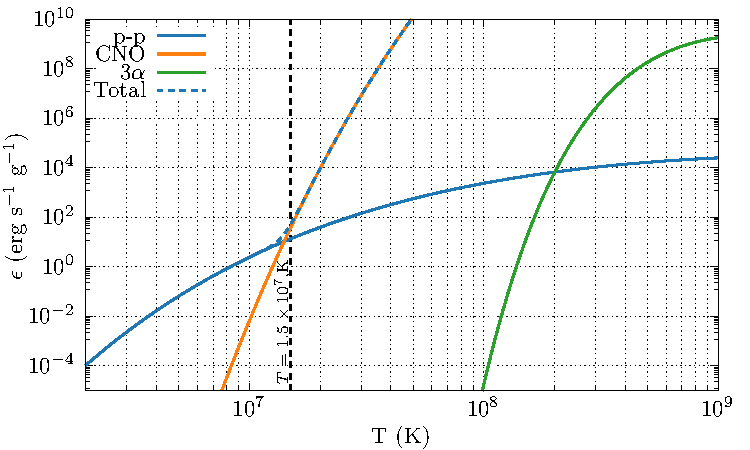
\includegraphics{assets/reaction-rate/reaction-solar.pdf}
  \caption[Reaction rates at the center of the sun]{Reaction rates from p-p, CNO and triple-$\alpha$ fusion processes at the centre of the sun. At the solar core temperature of \SI{1.5e7}{\kelvin} only 10\% of the energy produced from fusion is through the CNO cycle. At higher internal temperatures the CNO cycle rapidly becomes dominant due to its stronger temperature dependence. The $3\alpha$ process does not occur in the solar core, but becomes the dominant fusion process in high-mass stars leaving the main sequence. Solar abundances and a core density of \SI{150}{\gram\per\centi\metre\cubed} are assumed.}
\end{figure}


\subsection{Stellar winds}

% Influence of OB stars on surrounding environment, outsized influence etc.
The luminosities and temperatures of high-mass stars also drive extremely fast stellar winds through radiative line driving.
These winds are on the order of $10^{10}$ times stronger than winds from stellar-mass stars, and punch holes clean into the interstellar medium (ISM), forming wind-driven bubbles and champagne cork flows, as well as perturbing GMCs, allowing for further star formation.

The study of stellar winds, of course, is quite hard from our vantage point on earth.
Sampling the winds themselves is difficult due to the vast, inconvenient distances involved in sending a probe to collect the rarefied material from our stellar neighbourhood.
Additionally, the bubble blown from our own suns stellar wind makes collection even more difficult, leaving the heliosphere is no easy feat either, just ask the Voyager probes.
We instead derive the properties of these extrasolar winds from spectrography, with the adsorption and emission spectra of the winds betraying their composition.
The velocity of these winds can be determined in much the same manner, through the Doppler shift of these emission lines.
Early observations of stellar winds centred around the star P Cygni, the earliest known example of an evolved Luminous Blue Variable (LBV) star.
the presence of peaks and throughs in the profile of a spectral line such as H-$\alpha$ was the cause of some scientific curiosity.
This effect could only be explained by the presence of a shell rapidly expanding away from the star.
The troughs of this emission line corresponded to a blue-shifted adsorption lobe, from radiation passing through this shell, while the emission line itself corresponded to the expanding shell itself \parencite{bealsNatureWolfRayetEmission1929,lamersIntroductionStellarWinds1999}.
Observations of other stars typified this event, it was found that every star had a stellar wind, though the speed and quantity of the ejected material could vary by many orders of magnitude.

% Very basic 
In the simplest terms, we can describe a stellar wind as a spherical outflow from a star.
We can describe this outflow in terms of its mass loss rate, $\mdot$, the amount of material ejected from the star, as well as its terminal velocity, $\vinf$, or the maximum velocity a wind can obtain from its driving mechanism.
We can use these to determine a profile of the density of a stellar wind as a function of its distance, $\boldsymbol{r}$, from the star

\begin{equation}
  \rho_w = \frac{\dot{\text{M}}}{4 \pi v^\infty \boldsymbol{r}^2}, \label{eq:smoothwind}
\end{equation}

\noindent
where the star is a point source.
Whilst this barest description can give us some insight into how a wind behaves, we should discuss the driving mechanisms behind these winds, as well as the more complex models we use to describe them.

\subsubsection{Driving mechanisms}

\begin{table}[h]
  \centering
  % \resizebox{\textwidth}{!}{%
  \begin{tabular}{llll}
  \hline
  \multicolumn{1}{l}{Classification} & \multicolumn{1}{l}{$\dot M$} & \multicolumn{1}{l}{$v_\infty$} & \multicolumn{1}{l}{Mechanism} \\
  \multicolumn{1}{l}{}     & \multicolumn{1}{l}{\si{\solarmass\per\year}}         & \multicolumn{1}{l}{\si{\kilo\metre\per\second}}           & \multicolumn{1}{l}{}          \\ \hline
  Sun            & $10^{-14}$        & 400  & Thermal heating \\
  PMS & $10^{-4}-10^{-7}$ & 200-500 & Rotation \& magnetic fields \\
  Red Giant      & $10^{-7}-10^{-9}$ & 30   & Radiation pressure on dust grains        \\
  OB Star        & $10^{-7}-10^{-8}$ & \num{2500} & Radiation pressure \& line driving      \\
  Wolf-Rayet     & $10^{-5}$         & \num{1500} & Radiation pressure \& line driving       \\ \hline
  \end{tabular}%
  % }
  \caption[Stellar wind comparison]{Comparison of stellar winds emitted from various classification of star.}
  \label{tab:windcomp}
\end{table}

\begin{figure}[h]
  \centering
  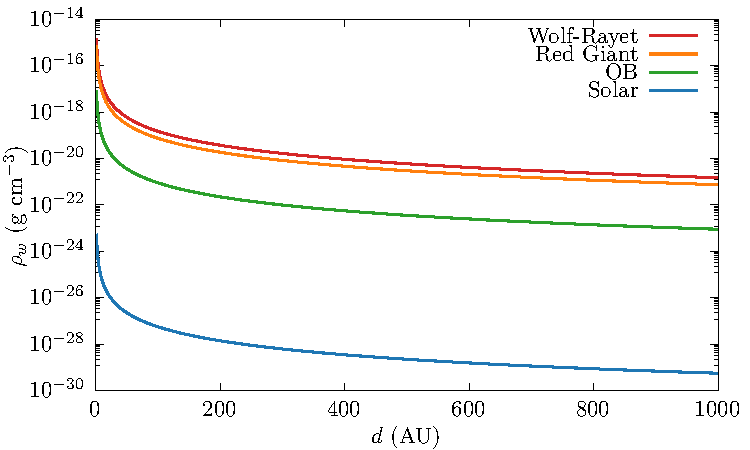
\includegraphics{assets/wind-comparison/wind-comp.pdf}
  \caption[$\rho_w$ comparison of main sequence winds]{Comparison of the densities of various main sequence winds using the parameters specified in table \ref{tab:windcomp}, wind densities are estimated using the smooth wind approximation described in equation \ref{eq:smoothwind}.}
  \label{fig:windrhocomp}
\end{figure}

\begin{figure}
  \centering
  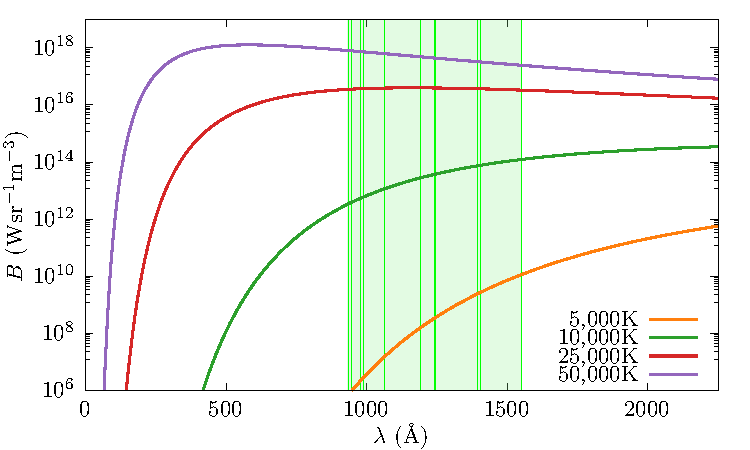
\includegraphics{assets/plancks-law/plancks-law.pdf}
  \caption[Planck's law radiance comparison with resonance lines]{Spectral radiance against wavelength for black body objects at various effective temperatures, $T_{\text{eff}}$, a series of wavelengths corresponding with important resonance lines in Table 1 of \textcite{lucy_mass_1970} have been included. As temperature increases the spectral radiance at resonance line wavelengths dramatically increases, with a minimum of 6 orders of magnitude difference between the effective temperatures of a solar equivalent main sequence star and an O-type main sequence or Wolf-Rayet star.}
  \label{fig:planck-comp}
\end{figure}

% Low mass stars

Low-mass main sequence stars, compared to other classes of star, have winds that are relatively thin, with a mass loss rate of $10^{-14} \, \si{\solarmass\per\year}$.
Along with their middling velocity of \SI{400}{\kilo\metre\per\second} this results in a wind density many orders of magnitude lower than other types of star (Fig. \ref{fig:windrhocomp}).
The reason for this comparatively feeble outflow is the driving mechanism.
The corona in stars with a convective envelope is approximately 3 orders of magnitude hotter than the stars photosphere, this hot corona exerts pressure on gas trapped within it, causing it to be expelled from the star.
As this method is thermally driven, and does not expel gas from the envelope directly, this explains the comparative weakness.
In fact, winds from red dwarfs are found to be markedly denser, but the mechanisms behind the driving force are less well understood.
% Evolved low-mass stars
As low-mass stars evolve and leave the main sequence, swelling into red giants, the surface gravity of the star decreases dramatically.
Furthermore, as the star expands and cools, dust condenses and forms in the photosphere.
These dust grains adsorb photons more readily than ions and atoms through Thompson scattering, and can adsorb a broad range of wavelengths due to their size.
Radiation pressure then drives these dust grains away, if the gas is sufficiently coupled to the wind this is driven away too, in the form of a dense, optically thick, barely supersonic wind
\parencite[Ch.~5]{lamersIntroductionStellarWinds1999}.
The mass loss rates of these stars are extremely high, no lower than $10^{-7} \, \si{\solarmass\per\year}$ and as high as $10^{-5} \, \si{\solarmass\per\year}$ but have velocities on the order of $10-100 \, \si{\kilo\metre\per\second}$.

% High mass stars

By the 1970s the winds of early-type stars had been categorised, finding mass loss rates between $10^{-8}$ to $10^{-5} \, \si{\solarmass\per\year}$ and wind velocities of \num{600} to \SI{3500}{\kilo\metre\per\second}.
Additionally, it was found that the mass loss rate of these stars was approximately proportional to the luminosity ($\mdot_\star \propto L_\star^{1.1}$) \parencite{cassinelliStellarWinds1979}.
This strongly suggested that the driving mechanism of these winds was based on radiation pressure, though thompson scattering would not be a sufficiently efficient process to drive winds of this magnitude.
Furthermore, coronal heating and dust driving mechanisms were not possible, due to a lack of a convective envelope and lack of significant dust build up in the envelope, respectively.

\subsubsection{Line-driven wind theory}
\label{sec:cak}

% Line driven wind theory 
Instead, wind driving through resonance lines was proposed.
A photon with an energy equal to the excitation energy of an emission line of an ion in the wind is adsorbed, exciting the ion.
This ion then de-excites over a timescale of $10^{-8} \, \si{\second}$, emitting a photon at a random angle relative to the radial direction relative to the star, $\alpha$.
This emission of a photo produces a recoil force on the ion, resulting in a change in the radial velocity, $\Delta v\rms{r}$, such that:

\begin{equation}
  \Delta v\rms{r} = v\rms{r}'' + v\rms{r}' - v\rms{r} = \frac{h\nu_0}{mc} \left(1-\cos \alpha \right),
\end{equation}

\noindent
where $v\rms{r}'$ is the ions radial velocity after the photon adsorption, $v\rms{r}''$ is the ions radial velocity after photon emission and $\nu_0$ is the frequency of the resonating photon.
Compared to Thompson scattering, resonance lines are 6 orders of magnitude more opaque, making it a much more efficient process
\parencite[Ch.~8]{lamersIntroductionStellarWinds1999}.
This driving force occurs more readily with elements with a large number of resonant lines, heavier ions such as C, N, O and Fe group elements adsorb the photons.
Lighter elements such as H and He are instead carried along via Coulomb forces, coupled to the heavier elements so long as the medium is sufficiently dense.

But why is this effect not observed in lower mass stars?
Firstly, resonance lines in heavier elements are comparatively high energy, requiring 
For instance, the C III resonance line has an energy of \SI{12.69}{\electronvolt}, therefore a photon requires a wavelength of \SI{977}{\angstrom} in order to be adsorbed (Fig. {\ref{fig:planck-comp}}).
Secondly, photons would only be adsorbed over a narrow range of frequencies.
This would inhibit efficient momentum transfer from UV photons without Doppler shift, as the outflow from the star has a distribution of radial velocities this results in a greater chance of resonance line adsorption.
If we were to observe the outflow of a massive wind we would therefore see a relatively low velocity component of the wind close to the star; once the wind reaches a certain critical velocity.
At a certain point we would observe a significant and rapid increase in the velocity of the wind, as the influence on adsorption due to Doppler shift results in the wind becoming much more opaque to UV photons.
Eventually we would observe the wind reaching a terminal velocity, due to a decrease in photon flux from the inverse square law and the outflow becoming more diffuse as it spreads away from the star \parencite[Ch.~10]{maciel_hydrodynamics_2014}.
This can be seen in Fig. \ref{fig:cak-vel}, where the velocity increases sharply at a distance $(R/R_\star) - 1 > 10^{-3}$ as the wind begins to rapidly accelerate away from the star as opacity increases - with a corresponding decrease in wind density.

\begin{figure}
  \centering
  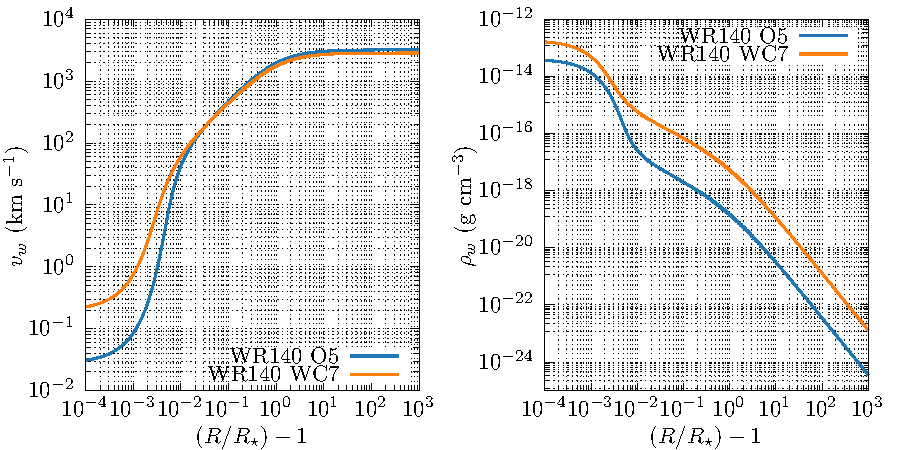
\includegraphics[]{assets/cak/vel.pdf}
  \caption[Radiative line driving velocity and density profile]{Velocity and density profiles of the WR and OB stars in the WR140 system. Acceleration is gradual until $(R/R_\star) - 1 > 10^{-3}$, where wind opacity drastically increases due to Doppler shift. The model uses the Castor, Abbott and Klein formalism, with the CAK parameters of the stars estimated to be $k = 0.37$, $\alpha = 0.60$ for the O4-5 star and $k = 0.48$, $\alpha = 0.57$ for the WC7 star.}
  \label{fig:cak-vel}
\end{figure}

Theories of radiation pressure being the main driving force for massive stars was first considered by astronomers in the early \nth{20} century, and was first proposed by \textcite{sahaRadiationPressureQuantumTheory1919}.
Later, \textcite{milnePossibilityEmissionHighspeed1926} who predicted that after an initial acceleration phase from an ions emission lines, Doppler shift would be sufficient for continuum photons frequencies to match the resonant lines - causing a much greater impulsive force.
Early calculations of the force on stellar winds due to resonance lines by \textcite{lucy_mass_1970} found initial estimates for the mass loss rate based on a series of resonance line in the C, N, Si and S species of ions.
However, these were found to underestimate the mass loss by approximately two orders of magnitude.
This is in part due to the models simplicity, due to limitations in both computing power and available data, as the force due to interaction of resonance lines with continuum photons were considered.
The first major breakthrough was with more complex models demonstrated by Castor, Abbott and Klein (\citeyear{castor_radiation-driven_1975}; CAK).
The CAK model computed line forces from all emission lines in the C III ion, after estimating the line force from other ions by scaling the results of this calculation an estimate of mass loss rates for hot stars was calculated to within a factor of 3 of observational results.
A much more complex emission line model developed by \textcite{1982ApJ...259..282A} involved the calculation of the force from a startling \num{250000} lines, however, this was found to be less accurate than the original CAK model!
This led to improvements on the approximations and assumptions made by the CAK model, namely the finite disk correction factor
\parencite{friend_theory_1986,pauldrachRadiationdrivenWindsHot1986}.

\subsection{Evolved early-type stars}
\label{sec:evolvedstars}
% Evolution and fate of massive stars, evolution, depletion of hydrogen products, then onto helium burning
Unfortunately for the most massive stars, pesky limitations such as the conservation of energy severely curtail their lifespans.
Despite being anywhere from 3 to 5 orders of magnitude brighter, the most massive stars typically have between 1 and 2 orders of magnitude more fuel.
As such, they simply cannot compete with the ten billion year lifespan of our sun, or red dwarfs, which can have lifespans in the \emph{trillions} of years!
% Luminosity lifetime relation
In order to approximate the main sequence lifespan of a massive, early-type star we must make some assumptions.
We can assume the main sequence lifespan of a star is based on the amount of available hydrogen in the star and the fusion rte of the star, we can estimate that this lifespan, $\tau_\star$, through the equation:

\begin{equation}
  \tau_\star \approx \frac{\mass_\star}{\lumin_\star} ,
\end{equation}

\noindent
where $\mass_\star$ is the mass of the star and $\lumin_\star$ is the luminosity of the star.
Through observation we can determine an approximation of the mass-luminosity relation \parencite[139]{salarisEvolutionStarsStellar2005}, such that:

\begin{equation}
  \frac{\lumin_\star}{\lumin\sol} \propto
  \begin{cases}
    (\mass_\star/\mass\sol)^{2.6} , & \text{if } \SI{0.2}{\solarmass} \lesssim \mass_\star \lesssim \SI{0.5}{\solarmass} \\
    (\mass_\star/\mass\sol)^{4.5} , & \text{if } \SI{0.5}{\solarmass} \lesssim \mass_\star \lesssim \SI{2}{\solarmass} \\
    (\mass_\star/\mass\sol)^{3.6} , & \text{if } \SI{2}{\solarmass} \lesssim \mass_\star \lesssim \SI{20}{\solarmass} .
  \end{cases}
\end{equation}

\noindent
We can then make the following estimate for the main sequence lifespan of a massive star:

\begin{equation}
  \label{eq:mass-lifespan}
  \tau_\star \approx \tau\sol \left(\frac{\mass_\star}{\mass\sol}\right)^{-2.6}.
\end{equation}

\noindent
Assuming a solar lifespan of $\tau\sol = \SI{10}{\giga\year}$ we find through Eq. \ref{eq:mass-lifespan} that a typical O-type star with a mass of \SI{20}{\solarmass} is $\sim \SI{4.14}{\mega\year}$.
It takes the sun approximately \SI{230}{\mega\year} to orbit the galaxy, making its ``age'' approximately 19 galactic ``years'' old. Continuing this train of thought, even the least luminous early type star does not make it to its first birthday!

% == New para

% Running out of fuel, schonberg
Eventually, the hydrogen in the core is completely exhausted, leaving an inert helium core with a hydrogen envelope surrounding it.
Near the edge of the core, the temperature is still sufficient for hydrogen to burn, with energy production in the star relegated to a shell surrounding the inert core.
As the star transitions from core to shell H-burning \textcite{schonbergEvolutionMainSequenceStars1942} determined that the core and envelope temperature gradient is radiative, with an isothermal stratification.
They went on propose tht there is a limiting factor on the stable core size of a star.
Above this \emph{Sch{\"o}nberg-Chandrasekhar} limit ($q\rms{SC}$) the core contracts on the KH timescale (Eq. \ref{eq:khtime}), with the limit determined by a ratio the mean molecular mass, $\mu$, of the envelope and the core, such that:

\begin{equation}
  q\rms{SC} \equiv \left(\frac{\mass\rms{core}}{\mass\rms{tot}}\right)\rms{SC} = 0.37 \left(\frac{\mu\rms{env}}{\mu\rms{core}}\right)^2 .
\end{equation}

\noindent
For a star of solar composition we find $q\rms{SC} \sim 0.08$
\parencite[Ch.~5]{salarisEvolutionStarsStellar2005}.
For low-mass stars, this collapse timescale is extremely slow, instead the star expands into an asymptotic giant branch (AGB) star, continuing shell burning until the material is exhausted
\parencite{beechSchoenbergChandrasekharLimitPolytropic1988}.
This leaves behind a degenerate helium core in the form of a white dwarf, which continues to contract and emit radiation through KH processes\footnote{Finally! Kelvin was right!}.
For massive stars the ratio of core mass to total mass is significantly higher, exceeding the Sch{\"o}nberg-Chandrasekhar limit.
Instead, the core collapses, compressing and heating rapidly, eventually reaching temperatures sufficient for the commencement of helium burning through the Triple-$\alpha$ (3$\alpha$) process:

\begin{equation}
  \begin{alignedat}{3}
    \atom{He}{4}{2} + \atom{He}{4}{2} & \rightleftarrows \atom{Be}{8}{4} && ~~ - \SI{0.09}{\mega\electronvolt} \\
    \atom{Be}{8}{4} + \atom{He}{4}{2} & \rightarrow \atom{C}{12}{6} + 2\gamma && ~~ + \SI{7.37}{\mega\electronvolt} 
  \end{alignedat}
\end{equation}

\noindent
Which can also produce a small amount of oxygen with an additional $\atom{C}{12}{6} + \atom{He}{4}{2}$ interaction.
The endothermic component of the 3$\alpha$ process, as well as the short reaction time prevents it from occurring in any reasonable quantity until core temperatures are in the order of hundreds of millions of Kelvin
\parencite[Pt.~6]{kippenhahnStellarStructureEvolution2012}.
The reaction rate of the 3$\alpha$ process is proportional to $T^{40}$, a truly extreme dependence, which can result in truly \emph{staggering} rates of energy production.
However, this process is far less energy efficient than hydrogen burning processes, releasing an order of magnitude less energy per nucleon (Table \ref{tab:reactionrates}).
At this point, however, the fate of the star is already sealed, it hurtles off of the main sequence like a 1966 Ford Thunderbird from the edge of the Grand Canyon\footnote{See \emph{Thelma and Louise} (1991) dir. Ridley Scott.}.

% Brief explanation of evolution track
As this fusion process begins, it augments the rapidly thinning hydrogen burning shell.
Enormous photon flux drives the the outer envelope away, shifting the calculus of hydrostatic equilibrium from contraction to expansion, and the star expands into a supergiant star or a luminous blue variable (LBV) star.
Over the course of this giant phase, the most massive of early-type stars can enter a short lived, particularly violent stage of their lives, and transition into a Wolf-Rayet star - one of the cruces of this thesis.

\subsubsection{Wolf-Rayet stars}
\label{sec:wrtype}

\begin{figure}[h]
  \centering
  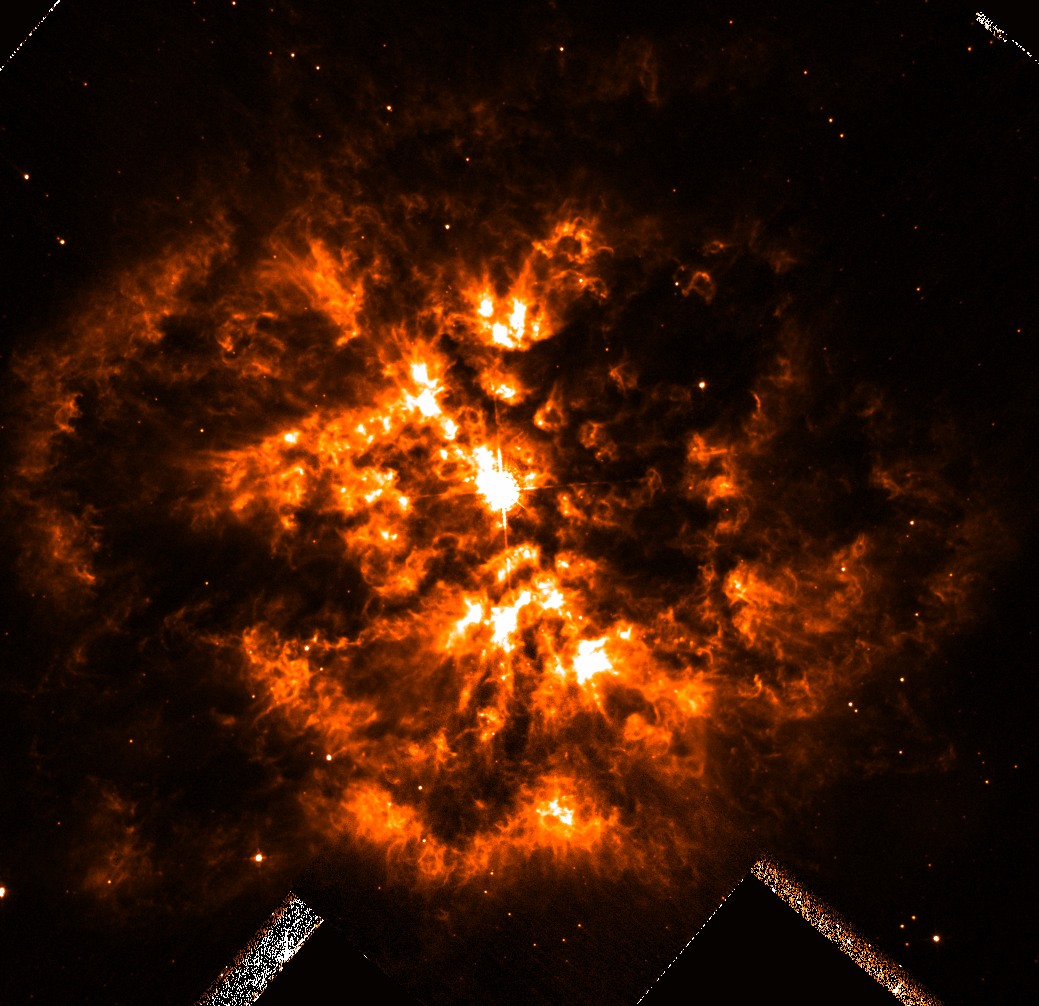
\includegraphics[width=4in]{assets/WR124.png}
  \caption[\textit{M1-67 nebula around WR 124 \parencite{2010ApJ...724L..90M}}]{Reduced Hubble WFPC2 data of the WN star WR 124, its extreme mass loss is currently producing the ejecta nebula M1-67 \parencite{2010ApJ...724L..90M}.}
  \label{fig:wr124}
\end{figure}

\textcite{crowther_physical_2007}

\begin{equation}
  \begin{alignedat}{3}
    \text{O} & \rightarrow \text{LBV/RSG} \rightarrow \text{WN} \rightarrow \text{WC} \rightarrow \text{SN 1b} && \text{ for } 25 \, \si{\solarmass} < \text{M}_{\text{WR}} < 40 \, \si{\solarmass} \\
    \text{O} & \rightarrow \text{LBV} \rightarrow \text{WN} \rightarrow \text{WC} \rightarrow \text{SN 1c} && \text{ for } 40 \, \si{\solarmass} < \text{M}_{\text{WR}} < 75 \, \si{\solarmass} \\
    \text{O} & \rightarrow \text{WN(H-rich)} \rightarrow \text{LBV} \rightarrow \text{WN} \rightarrow \text{WC} \rightarrow \text{SN 1c} && \text{ for } \text{M}_{\text{WR}} > 75 \, \si{\solarmass} 
  \end{alignedat}  
\end{equation}




% == New para

% Wolf-Rayet stars

% Brief background

% Explanation, history

% Brief explanation of wind driving, Eddington limit

% WC/WN/WO stars

% Why WC stars are only covered in this thesis, dust prod.

As we now know, Wolf-Rayets\footnote{Abbreviated to WR.} are evolved forms of O-type stars, and are a short lived component of the life-cycle of massive stars, typically lasting for around \num{5e5} years \parencite{crowther_physical_2007}.
Despite this relatively transient length of this stage, the influence of a WR star on its local medium is extremely outsized.
WR stars in particular are known for having dense, fast winds, typically between 2 and 3 orders of magnitude than their main sequence O-type progenitors, with mass loss rates on the order of $10^{-5} \, \si{\solarmass\per\year}$ and wind velocities of $\num{1.5e3} \, \si{\kilo\metre\per\second}$.
This extremely dense wind is driven by the highly energetic helium burning core, which is luminous enough as to drive away the outer layers of the stars envelope, exposing the core.
The observed spectroscopic lines are due to heating of the envelope from the core, which is enriched with by-products of hydrogen and helium burning, the lack of hydrogen lines is due to the stars evolved nature, as all the hydrogen has been burned, there is simply nothing left to observe!

%Subcategorising wolf-rayets into WN, WC and WO

Wolf-Rayet stars can be subcategorised through spectroscopic observation, which indicates enrichment in a particular element, the 3 major sub-types, WN, WC and WO are defined by their strong nitrogen, carbon and oxygen lines respectively.
The important distinction between WN and WC/WO stars is that WN stars are enriched through hydrogen burning, whilst WC and WO are enriched through the by-products of helium burning \parencite{vinkVeryMassiveStars2015}.

% WR star subcategorisation and evolution
As a Wolf-Rayet continues to lose its envelope, additional products of fusion processes are dredged up from the centre of the star.
In the case of the WN sub-type, the broad nitrogen lines correspond to the outer layer of the envelope, enriched through the CNO process; after this outer envelope is cast off, the remainder of the envelope exhibits carbon and oxygen lines, indicating enrichment from the triple-$\alpha$ process.
Finally, the star evolves further and the innermost region of the envelope is revealed, observed as the strong oxygen lines of a WO sub-type \parencite{neugentWolfRayetContent2019,oswaltPlanetsStarsStellar2013}.

%//TODO this needs rewriting

As an O-type star transitions to a Wolf-Rayet, it typically undergoes an intermediary LBV or RSG stage as helium burning begins, this is mass dependent, with the various transitional states described by \cite{crowther_physical_2007}:

\begin{subequations}
  \begin{align*}
    \text{O} \rightarrow \text{LBV/RSG} \rightarrow \text{WN(H-poor)} \rightarrow \text{WC} \rightarrow \text{SN 1b} & ,~~ \text{for } 25 \, \si{\solarmass} < \text{M}_{\text{WR}} < 40 \, \si{\solarmass} \\
    \text{O} \rightarrow \text{LBV} \rightarrow \text{WN(H-poor)} \rightarrow \text{WC} \rightarrow \text{SN 1c} & ,~~ \text{for } 40 \, \si{\solarmass} < \text{M}_{\text{WR}} < 75 \, \si{\solarmass} \\
    \text{O} \rightarrow \text{WN(H-rich)} \rightarrow \text{LBV} \rightarrow \text{WN(H-poor)} \rightarrow \text{WC} \rightarrow \text{SN 1c} & ,~~ \text{for } \text{M}_{\text{WR}} > 75 \si{\solarmass} 
  \end{align*}  
\end{subequations}

%//TODO add binary formation mechanism paragraph

% subcategorisation through numerical system

%//TODO include table of approximate mass loss rates, numerical classification

% Wolf-Rayets in a binary
Wolf-Rayet stars are important in the context of this work due to their outsized influence within a WR+OB binary pair.
The WR component of a WR+OB binary has an outsized contribution in returning material to the ISM, whilst also dominating the dynamics of the system, with their winds completely overpowering those of their O-type neighbours.
In some cases, the dense, fast wind from the WR can collide with the much more tenuous wind from its partner, forming a strong shock, and a variety of fascinating effects.
However, I wouldn't want to spoil too much too soon, but you can skip ahead to section \ref{sec:cwb}, where this phenomena is covered in more detail.
%//HMM This may be a bit too jovial!

\subsubsection{The death of a star}

% Continued evolution, carbon burning
The star, unconcerned with shedding a significant portion of its mass, continues its death march\footnote{I understand that this section has taken a flair for the dramatic, but what \emph{isn't} dramatic about the death of a star?}.
The core contracts further, heating to temperatures in the range of $10^9 \, \si{\kelvin}$, carbon atoms are smashed together and burned, producing even heavier elements:

\begin{equation}
  \begin{alignedat}{3}
    \atom{C}{12}{6} + \atom{C}{12}{6} & \rightarrow \atom{Ne}{20}{10} + \atom{He}{4}{2} && + \SI{4.62}{\mega\electronvolt} \\
    \atom{C}{12}{6} + \atom{C}{12}{6} & \rightarrow \atom{Na}{23}{11} + p && + \SI{2.24}{\mega\electronvolt} \\
    \atom{C}{12}{6} + \atom{C}{12}{6} & \rightarrow \atom{Mg}{23}{12} + n && + \SI{2.60}{\mega\electronvolt}
  \end{alignedat}
\end{equation}

\noindent
These reactions salvage miniscule amounts of energy per nucleon, burning through the carbon in the core in a year.
% Neon burning, buildup of nuclear ash
The core continues to contract, more vigorous and less efficient fusion processes begin to pile up on each other.
The star burns its neon, then its oxygen, and then its silicon - the latter of which has a flurry of reaction modes that produce many different elements, burning through the entire reserves in about a day
\parencite[Ch.~6]{ryanStellarEvolutionNucleosynthesis2010a}.

% Iron
Finally, iron begins to deposit in the core of the star, all fusion processes at this point are endothermic, without any more fuel sources, the star truly collapses.
The core rushes inwards, accelerating to an appreciable fraction of the speed of light, with truly unimaginable densities and temperatures in excess of \SI{100}{\giga\kelvin}\footnote{I can state a temperature of \SI{100}{\giga\kelvin} but can you really \emph{imagine} it? Can anyone really comprehend that kind of temperature?} protons capture electrons, forming neutrons and emitting copious amounts of neutrinos.
As the core tumbles inwards, neutron degeneracy suddenly halts the collapse, the near-relativistic core material suddenly forms a shock wave, jumping to more absurd temperatures and pressures.
The rebounding material forms a Type II core-collapse supernova, ejecting heavy elements - formed through neutron capture - into an unsuspecting universe, leaving behind a neutron star, the remnant of the electron capture mechanism from the original inward dive\footnote{Randall Munroe of \href{https://what-if.xkcd.com/73/}{\texttt{XKCD}} has stated a good rule of thumb for supernovae that I tend to follow: ``However big you think supernovae are, they're \emph{bigger} than that.''}.

In the case of collapsing Wolf-Rayet stars, however, this can go further.
Neutron degeneracy is insufficient to halt the collapse and the core collapses into a black hole.
The resultant jet of material from this hypernova\footnote{\emph{Bigger than bigger than that!}} makes up a gamma-ray burst (GRB), a phenomena that can threaten planets \emph{thousands} of light years from their point of origin.
We should stop here, however, as this section is more to provide context as to what early-type stars fundamentally are: violent, destructive, and awe-inspiring.
It seems absurd that these systems could produce anything as fragile as interstellar dust.

And yet they \emph{do} - as we will later discuss.

\section{Interstellar Dust}
\label{sec:dust}

% Observational history
For much of the history of astronomy, interstellar dust was not its own field, nor was it studied in significant detail - instead it was regarded as nothing but a \emph{nuisance}.
Early astronomy, of course, was limited to the visible light spectra, at these wavelengths dust \emph{is} in fact a nuisance, contributing nothing and extincting stars and the innermost depths of the galaxy.
The first population counts of stars at the turn of the \nth{20} century were hampered by this extinction, with \textcite{kapteynAbsorptionLightSpace1909} noting that:

\begin{quote}
  \textit{
    ``Undoubtedly one of the greatest difficulties, if not the greatest of all, in the way of obtaining an understanding of the real distribution of the stars in space, lies in our uncertainty about the amount of loss suffered by the light on its way to the observer.''
  }
\end{quote}

\noindent
The existence of dust grains was not considered until nearly a quarter of a century, with work by Robert J. Trumpler in 1930 concluding that the observed interstellar reddening effect could only be accounted for by small grains of cosmic dust.
As technology progressed and non-visible astronomy became possible, we were for the first time able to peer past these obscuring clouds, bypassing them entirely.
The scientific community also found that the interstellar dust itself was interesting on its own, leading to further categorisation and parametrisation of these dust grains in the 1960s and 1970s
\parencite[4-13]{whittetDustGalacticEnvironment2002}.

Interstellar dust, particularly in the case of small grains, is a loose collective of atoms and molecules held together by weak molecular bonds, typically only on the order of $10 \, \si{\angstrom}$ to $100 \, \si{\angstrom}$ in size.
These grains are typically formed from small, refractory dust cores around $5\,\si{\angstrom}$ across, in high density regions such as stellar atmospheres and dark interstellar clouds \parencite{spitzerPhysicalProcessesInterstellar2008}.
This initial accretion process can be quite rapid, as outflows from stars can be quite rapid, due to implantation of impinging carbon ions \parencite{zubkoPhysicalModelDust1998a}.
While the largest dust grains can be on the order of centimetres (in the case of protoplanetary disks), the initial grain size in this project that we will consider is approximately $50 \, \si{\angstrom}$.
There are a multitude of ways that these dust grains can grow and shrink, though only a few are considered in this work, due to either difficulty of implementation into our model or time constraints.
The first such mechanism for growth and destruction that will be discussed is grain-grain collision.
Grain-grain interactions are the most easily understood, in regions with sufficiently high dust grain number densities, collisions can occur between the grains.
The result of this interaction is dependent on the collision velocity between the grains.
Low velocity collisions result in grain mergers, where these grains will stick together.
An initial attractive force through van der Waals interaction will occur, bringing the grains into contact, upon collision the contact area will deform and flatten, allowing for the grains to coagulate and merge.
Grain-grain coagulation occurs at very low velocities, typically $<\SI{100}{\metre\per\second}$, but this threshold velocity is typically lower for smaller, more tightly bound grains
\parencite{chokshiDustCoagulation1993}.
At higher collision velocities these grains can simply bounce off of each other, doing very little damage outside of ablating some atoms off of the surfaces of the grains.
At high velocities still these grains can shatter and fragment each other, which in the case of high velocity shocks with large grains can result in the grains being completely pulverised, turning from an accretion process to the principle cause of dust destruction
\parencite{jonesGrainShatteringShocks1996,jonesDustDestructionProcesses2004}.

The most important method of destruction of dust for this project is grain-gas sputtering, this thermal interaction dominates dust destruction at all temperatures in shocks.
As an ion collides with a dust grain in a shock, the surface near the impact site is vaporised, this impact also drives a shock wave into the grain, which can melt and shatter parts of the grain.
Over time material is ablated off of the dust grain, causing it to shrink in radius, and eventually completely shattered.
In order to simulate this we must simplify and parametrise this into a model, we start by assuming that the dust grain is spherical.
As the gas collides with the grain, small amounts of the grain are vaporised and ejected from the surface, causing a reduction in grain radius, $a$, with a corresponding rate of radius change $\dot a$.
$\dot a$ can vary depending on the composition of the grain; for instance, grains composed of ice would be more readily vaporised by impacts than sturdier grains composed of carbon or iron.
In this spherical case the dust destruction rate is inversely proportional to the number density of the gas, as the grain will be destroyed faster if there are more gas-grain interactions, and proportional to the grain radius.
The dust destruction rate has a more complex dependency on the grain temperature, rapidly reducing below $10^6\, \si{\kelvin}$, and is found to be roughly flat above this temperature and to around \SI{3e8}{\kelvin} \parencite{tielens_physics_1994}.
We can therefore adopt a normalised grain lifespan $\tau\rms{d}$, which we can use to calculate the dust destruction rate in our simulations:

\begin{equation}
  \tau\rms{d} \equiv \frac{a}{\dot a} \approx \num{3e6} \frac{a}{n\rms{g}} \, \si{\year} , 
\end{equation}

\noindent
where $n\rms{g}$ is the gas number density \parencite{drainePhysicsDustGrains1979,dwekCoolingSputteringInfrared1996}.
The value of \SI{3e6}{\year} was chosen for this project as it is more typical of temperatures in the post-shock region of a WCR, between $10^6\,\si{\kelvin}$ and $10^7\,\si{\kelvin}$ (Fig. \ref{fig:grain-lifespan}).
How this destruction rate is implemented into the simulations for this project is discussed in more detail in Section \ref{sec:bodmas}.

\begin{figure}
  \centering
  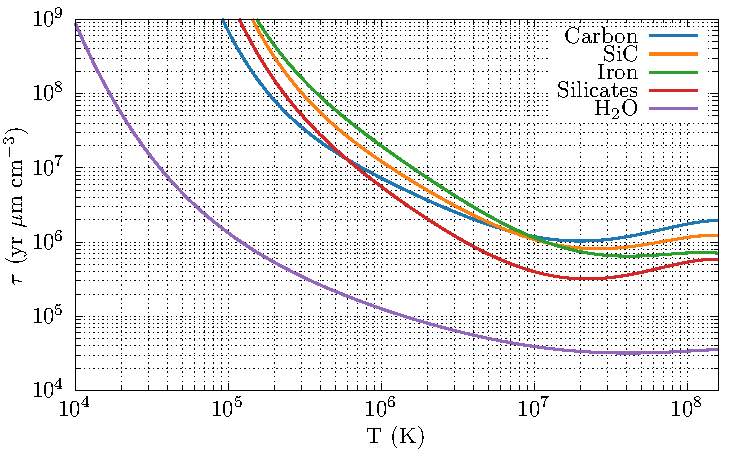
\includegraphics{assets/tielens-sputtering/sputter.pdf}
  \caption[Grain lifetime comparison]{Comparison of grain lifetimes for various interstellar dust species undergoing thermal sputtering in a fast interstellar shock. Lifetime is normalised to a grain radius of \SI{1}{\micro\metre} and a flow of \SI{1}{\gram\per\centi\metre\cubed} in a shock of solar abundance. Data is derived from \nth{5} order polynomial fits calculated in \textcite[Table~4]{tielens_physics_1994}.}
  \label{fig:grain-lifespan}
\end{figure}

% Dust-grain agglomeration 
As with grain-grain interactions, at lower velocities grains can impact onto grains or their nuclei and stick to the surface.
This steady accretion process be described in the form of a fairly simplistic model.
By considering a spherical grain moving through a flow of atoms with a number density $n\rms{a}$, a certain number of these atoms would collide and stick to the dust grain, this sticking probability is defined as $\xi$.
This sticking factor is found to be $\approx 1$ for neutral atoms\footnote{Though we adopt a more conservative value of $0.1$ due to the turbulent nature of the environments that are studied in this project.} \parencite{watsonAbundancesInterstellarMolecules1972}.
Above a threshold velocity, atoms fail to adhere to the grain surface, and at higher velocities still contribute to the sputtering process instead \parencite{spitzerPhysicalProcessesInterstellar2008}.
For this research, this threshold temperature was defined as \SI{14000}{\kelvin}.
If we model a grain of radius $a$, the cross section, $\sigma$, of the grain moving through the gas would be $\sigma = \pi a^2$.
In the case of a grain moving through a gas of composition $x$ and density $\rho_x$ where the grain is significantly larger than the atoms composing the gas, it is found that the rate of change in the grain mass, $dm\rms{gr}/dt$, is:

\begin{equation}
  \frac{dm\rms{gr}}{dt} = \sigma w_{x} \rho_{x} = \pi a^2 \rho_{x} w_{x} \xi_{x} ,
\end{equation}

\noindent
where $w_x$ is the RMS velocity of the gas.
The associated rate of change in grain radius, $da/dt$, is found to be:

\begin{equation}
  \frac{da}{dt} = \frac{w_x \rho_x \xi_x}{4 \rho\rms{gr}},
\end{equation}

\noindent
where $\rho\rms{gr}$ is the bulk density of the dust grain.

A myriad of other dust destruction processes exist, such as electron-grain and cosmic ray-grain interaction, but these are considered to be out of the scope of this project, and not influential in the case of a hot gas or dense post-shock environment
\parencite{jonesDustDestructionProcesses2004}.
Outside of shocks, dominant destruction processes include thermal and photo-dissociation methods.
UV light emitted from stars can ionise atoms on the surface of the grain, ejecting them from the surface, slowly ``boiling'' material from the grain.
This of course makes the premise of our project all the more curious, with so many mechanisms underpinning dust destruction, particularly in hot, dense environments, how come we observe significant dust production in Wolf-Rayet binary systems?

\subsection{Dust composition}

% Grain types being considered, amorphous carbon grains
The most important species of interstellar dust in this thesis are those composed of carbon.
$sp^2$- (graphite) and $sp^3$-bonded (diamond) dust grains have been detected from their characteristic emission lines, as well as hydrocarbon chains and Polycyclic Aromatic Hydrocarbons (PAHs).
Complex organic molecules have also also been detected in dusty environments, they are believed to have formed in the surface of dust grains, instead of forming within the ISM itself
\parencite{herbstComplexOrganicInterstellar2009}.
The primary dust detected in CWB systems is amorphous carbon grains, which are defined as grains with a mixture of $sp^2$- and $sp^3$-bonded carbon, with no structural order or polymerisation
\parencite{draine_interstellar_2003}.
% Other grain types, PAHs, ice and silicates
Other species of interstellar dust are abundant throughout the ISM; these species include water ice, silicate grains and Polycyclic Aromatic Hydrocarbons (PAHs).
However, these grain species have not been detected in dust producing CWB systems, in part due to element depletion, as WC stars are hydrogen-depleted.
Amorphous carbon grains are also markedly more resistant to erosion and fragmentation due to shocks than other grain types.
They are also more resistant to thermal sputtering as well, due to their higher sublimation temperature, this resilience is vital if they are to survive in the extreme conditions of a CWB system
\parencite{draineDestructionMechanismsInterstellar1979}.

\subsection{Radiation processes in interstellar dust}
\label{sec:dustcooling-background}

% Diffuse emission
Interstellar dust can be a significant factor in the cooling of its local interstellar medium through a series of continuum and line emission processes.
Collisional excitation and adsorption of photons can stochastically heat dust grains, this excess energy is then emitted in the form of near-infrared radiation \parencite{dwekCoolingSputteringInfrared1996}.
The radiative emittance of a dust grain can be approximated as a black body, and hence radiates in accordance with the Stefan-Boltzmann law:

\begin{equation}
  L = 4\pi r^2 \sigma T^4 , 
\end{equation}

\noindent
where $L$ is the grain luminance, $r$ is the grain radius, $\sigma$ is the Stefan-Boltzmann constant and $T$ is the grain temperature.
At sufficiently high gas densities this radiative process can become the dominant dominant cooling method in the ISM \parencite{wolfireNeutralAtomicPhases1995}.
In addition to this continuum emission, emission lines can also occur if characteristic vibrational modes in a grain lattice are excited, such as the silicate grain stretching and bending vibrational modes at \SI{9.7}{\micro\metre} and \SI{18.5}{\micro\metre} \parencite[212]{whittetDustGalacticEnvironment2002}.

\textit{Discuss the mathematics of this in more detail.}

% General cooling laws

\subsection{The importance of interstellar dust}
\label{sec:dustimportance}

We should ask ourselves, why are dust grains important enough to merit thousands of papers, and dozens of doctoral theses?
Over this short section we will attempt to explain in brief why dust grains so important.

% Interstellar dust grain species

Over 150 molecular species have been observed in the interstellar medium, with a surprisingly complex degree of organic chemistry; of the molecules with six or more atoms that have been detected, 100\% of these have been organic in nature.
Such complex organic molecules include benzene, acetone and ethanol, this degree of complexity should not necessarily be possible in interstellar gas-phase chemistry.
Instead, these organic species form on the surface of interstellar dust grains, with gas-phase chemistry accounting for simple molecule formation such as $\text{H}_2$ and $\text{CO}$
\parencite{herbstComplexOrganicInterstellar2009}.
The role of dust as the chemical refineries of the interstellar medium has a number of effects when it comes to star and planetary formation, as well as organic and pre-biotic chemistry throughout the universe.
It is no understatement to say that the universe would be remarkably different if interstellar dust was not so readily abundant.
% Coolant in collapsing gas clouds, stellar cycle
Dust grains are also vitally important in the star formation cycle.
As a Giant Molecular Cloud (GMC) collapses following perturbation, heat is generated, in the adiabatic case the increased temperature would provide a counterbalancing pressure on the collapsing cloud, forming a hydrostatic equilibrium and preventing the cloud from collapsing any further.
In the case of extremely massive clouds, this collapse can still occur as gravity will dominate, but this equilibrium dictates the minimum mass for a cloud to collapse into a protostar.
As such, for all but the most massive stars to form, energy must be lost in the form of radiation
\parencite{ward-thompsonIntroductionStarFormation2011}.
As radiative cooling from dust grains is extremely efficient in cold, dense environments, this mechanism is well-suited for the environment of a GMC.
In addition to cooling through rotational mechanisms of simple molecules in the gas-phase of the medium, these processes sufficiently cool the GMC, allowing for further collapse.
In addition, dust grains would also provide a replenishing source of cooling molecules such as CO and OH through non-thermal grain desorption processes.
The presence of dust grains within a GMC therefore strongly influences the minimum mass of stars
\parencite{williamsChemistryCosmicDust2015}.

% Planetary formation
Interstellar dust is also crucial for the formation of planets.
Collision between refractory dust grains is the first stage of planetesimal formation, within the protoplanetary disk, low velocity collisions between micron-sized grains can occur, causing these grains to stick and rapidly accrete.
If local region of the disk is gravitationally instable, these small grains will form a gravitationally bound cluster, and contract over time into a planetesimal, afterwards, rapid accretion of other planetesimals gives rise to the formation of both rocky planets and gas giants
\parencite{apaiProtoplanetaryDustAstrophysical2010}.
Dust is also a regulator of opacity, which determines the temperature structure and composition of the protoplanetary disk.
Finally, and perhaps most importantly to the reader, the complex organic molecules produced in the dust grain are pre-biotic precursors to life
\parencite{birnstielDustEvolutionFormation2016}.

As the role of interstellar dust in star and planet formation, as well as the long-term implications of the formation of life in the universe are \textit{slightly} out of the scope of this project, I will stop here, but it is always interesting to consider the repercussions of the topics that you research.

\section{Colliding Wind Binary Systems}
\label{sec:cwb}

Colliding Wind Binaries (abbreviated hereon to CWBs), in opposition to all known laws of astrophysical nomenclature, is a easy to understand term - it is a binary system where stellar winds from the member stars undergoing collision.
Unfortunately, the simplicity of the systems ends here, CWB systems are very poorly understood phenomena, due to a variety of factors that this section will discuss.

\subsection{History of CWB observation}

%History and classification, useful sources in Stevens & Pollock 1994 

Early observations beyond visual spectrum led to the discovery of many new astrophysical phenomena, one such discovery were extremely bright and variable thermal X-ray sources.
Many of these early galactic X-ray sources were found to be compact objects, and many more contained the characteristic spectral lines of a Wolf-Rayet star.
While single Wolf-Rayet stars are capable of producing X-ray emission, this is typically much dimmer than what was being observed 
\parencite{sewardXraysEtaCarinae1979}.
The existence of CWB systems were independently proposed by \textcite{prilutskii_x_1976} and \textcite{cherepashchukDetectabilityWolfRayetBinaries1976}, 
they proposed that significant and variable X-ray flux would result from the collision between two stellar winds, as these winds collide the gas becomes shocked and heated to temperatures on the order of \SI{1e8}{\kelvin}, hot enough to emit an appreciable quantity of X-rays.
The X-ray variability can also be explained as a result of the orbital properties of the systems, X-ray variability would result from the following effects:

% This may need to be expanded on or changed
\begin{itemize}
  \item Eccentricity in the orbits of the systems, leading to differing shock intensity and changing of the shock geometry, changing the fraction of the winds being shocked.
  \item Edge-on orbits resulting occlusion of x-rays by the stellar wind from each star. 
  \item Face-on orbits resulting in photospheric eclipses.
\end{itemize}

\noindent
Such effects could not be produced within a single star system \parencite{pittard_x-ray_1999}.
Further research by \textcite{pollockEinsteinViewWolfRayet1987} also found that single WR stars were typically faint, with the brightest X-ray emitting WR stars being confirmed to within massive binaries.
WR+OB systems were also found to be the brightest of such objects, while OB+OB binaries with significant X-ray flux were observed, these were typically less luminous.
% Early work categorising, using gamma 2 vel and V444Cyg
Early work was more concerned with X-ray observation, in particular the systems $\gamma^2$ Velorum and V444 Cygni, which were noted in particular as prototypical CWB systems by \textcite{prilutskii_x_1976}.
% Analysis pollock 1987 determined binary systems\cite{pollockEinsteinViewWolfRayet1987} 
Later, infrared observations of these systems found another, more curious attribute, a significant excess correlating to dust formation around these systems \parencite{williamsInfraredPhotometryLatetype1987}.
This will be discussed in more detail later in this section, but needless to say this phenomena is puzzling, as fragile grains of interstellar dust would not survive for long in the outflow of a WC star, due to the high wind temperatures and immense UV flux.
Because of this, dust growth was speculated, and later confirmed, to occur within the Wind Collision Region, the topic of the next section of this thesis.

\subsection{The Wind Collision Region}
\label{sec:wcr}

\begin{figure}
  \centering
  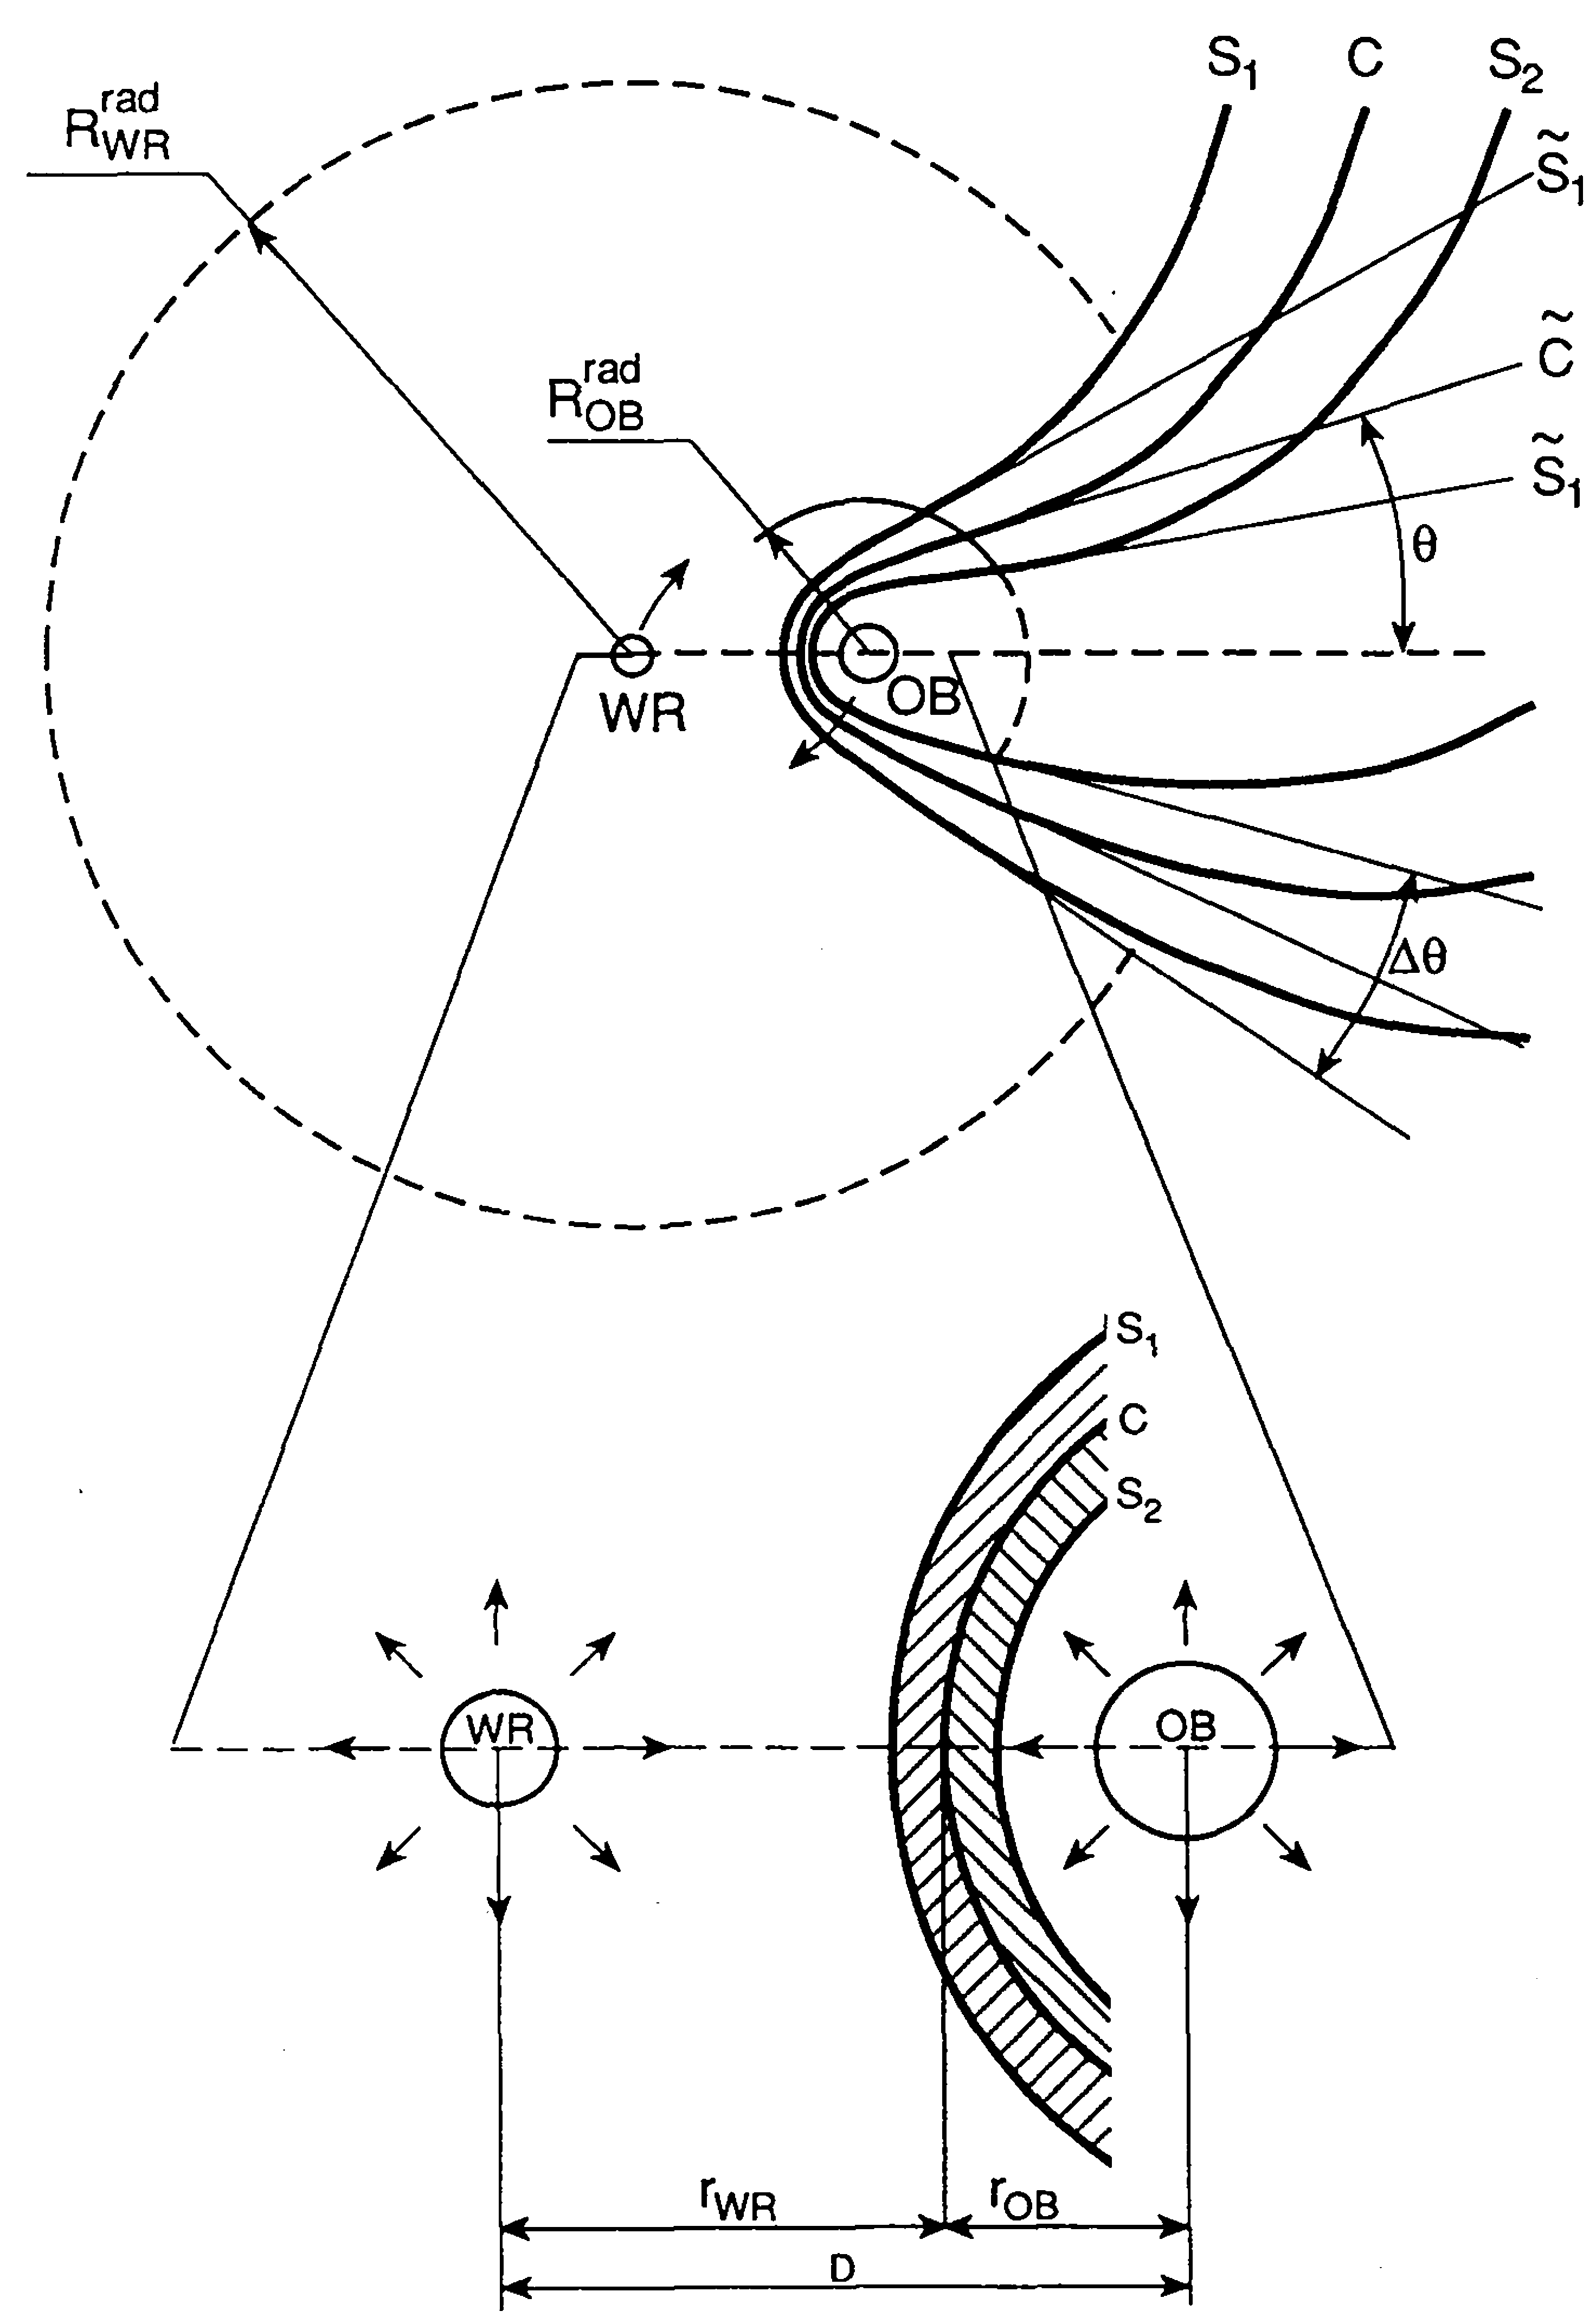
\includegraphics[width=3in]{assets/cwb-diagrams/eichler.png}
  \caption[\textit{A diagram of the Wind Collision Region \parencite{eichler_particle_1993}}]{A diagram of a typical Wind Collision Region inside a WR+OB CWB system. The $S_1$ and $S_2$ surfaces denote the shock waves from the primary and secondary winds respectively, and $C$ denotes the contact surface. The surfaces $\widetilde{S}_1$, $\widetilde{S}_2$ and $\widetilde{C}$ represent conic approximations of their corresponding surfaces at intermediate distances from the OB star. The region of stellar wind collision is hatched in the bottom diagram \parencite{eichler_particle_1993}.}
  \label{fig:wcr-diagram}
\end{figure}

\begin{figure}
  \centering
  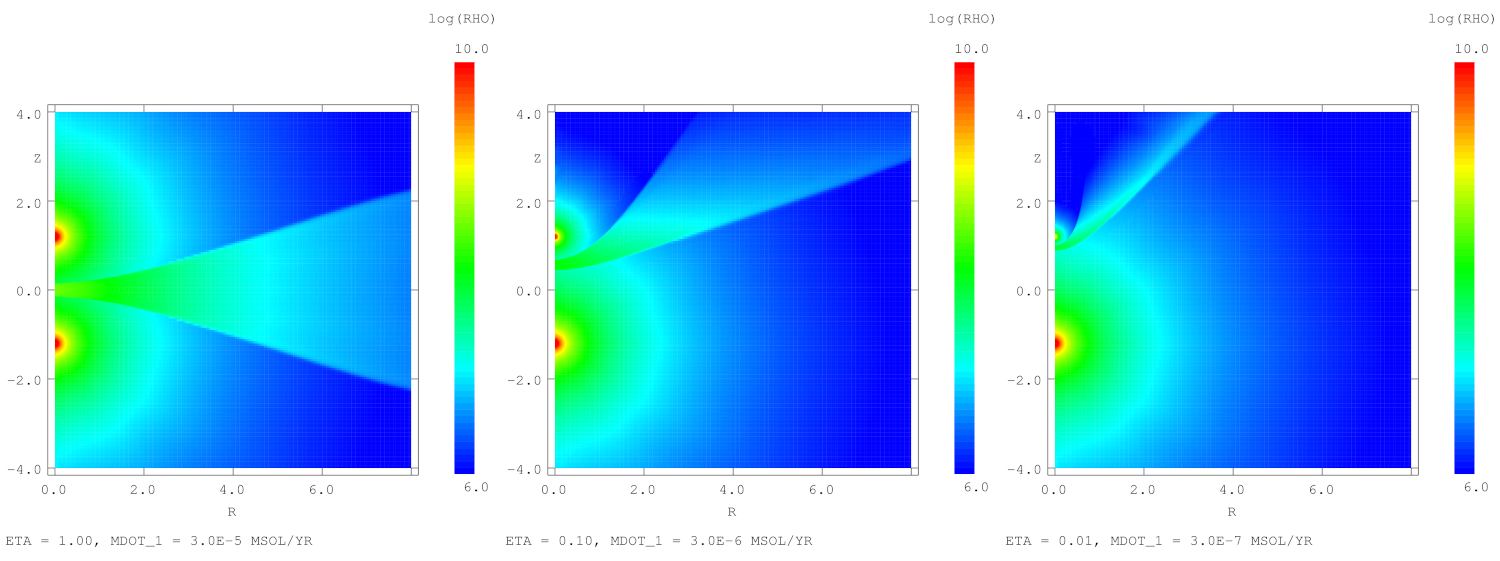
\includegraphics[width=6in]{assets/cwb-diagrams/eta.png}
  \caption[Comparison of wind momentum ratio, $\eta$, on WCR strtucture]{2D axisymmetric hydrodynamical simulations of CWB systems with wind momentum ratios of \num{1}, \num{0.1} and \num{0.001}. Momentum ratio is varied by changing the mass loss rate of the second star, $\dot{\text{M}}_2$. As $\eta$ decreases, the WCR begins to wrap itself around the secondary star.}
  \label{fig:wcr-eta}
\end{figure}

% What is this region
The Wind Collision Region (WCR) is the most violent and turbulent region of a CWB system, a region of high densities and even higher temperatures.
If the interacting stellar winds are dense as they begin to interact, a shocked region of plasma in excess of \SI{1e8}{\kelvin} is formed, the winds rapidly decelerate from hypersonic to subsonic, liberating an enormous amount of mechanical energy, on the order of \SI{1e3}{\solarluminosity}.
As previously discussed, this is the engine that drives the significant X-ray flux observed by astronomers in the 1970s, as well as other thermal and non-thermal emissions from the UV up to gamma rays \parencite{eichler_particle_1993,grimaldoProtonAccelerationColliding2019}.
As wind enters from either side of the wind collision region, it passes through a shock wave, and flows towards the centre of the wind collision region at the contact discontinuity, $C$ (Fig. \ref{fig:wcr-diagram}).
The wind behind the shock is driven by a combination of thermal pressure from the outflowing stellar wind, as well as the significant momentum the wind carried before being shocked \parencite{stevens_colliding_1992}.

The geometry of the WCR is influenced strongly by the wind parameters of both stars, the most important of which is the wind momentum ratio, or $\eta$, which we define as:

\begin{equation}
  \eta = \frac{\dot M_\text{OB} v^\infty_\text{OB}}{\dot M_\text{WR} v^\infty_\text{WR}},
\end{equation}

\noindent
where $\dot{\text{M}}_\text{WR}$ and $v^{\infty}_\text{WR}$ denotes the mass loss rate and wind terminal velocity of the primary, typically Wolf-Rayet star and $\dot{\text{M}}_\text{OB}$ and $v^{\infty}_\text{OB}$ denotes the mass loss rate and wind terminal velocity of the OB partner \parencite{usov_stellar_1991}.
A lower value of $\eta$ indicates a more unbalanced wind, with wind momentum ratio of \num{0.01} or lower being common for a typical WR+OB system.
Additionally, if $\eta = 1$, we observe a sheet of interacting plasma flowing away from the system perpendicular to the orbital plane.
In the case of a system where one stars momentum is significantly larger than the other, we observe the WCR extend and envelop the OB star, forming an approximately conical surface extending away from the Wolf-Rayet star (Fig. \ref{fig:wcr-eta}).


As the wind becomes more and more imbalanced, the contact discontinuity moves closer to the OB partner, this can be estimated with the equation:

\begin{equation}
  r_\text{WR} = \frac{1}{1+\eta^{1/2}} d_\text{sep} , ~~~ r_\text{OB} = \frac{\eta^{1/2}}{1+\eta^{1/2}} d_\text{sep} ,
\end{equation}

\noindent
where $r_{WR}$ is the distance from the WR star to the contact discontinuity, $r_\text{OB}$ is the distance from the OB star to the contact discontinuity and $d_\text{sep}$ is the orbital separation distance of the stars.

% Conic approximation


\begin{equation}
  \theta_c \simeq 2.1 \left(1 - \frac{\eta^{2/5}}{4}\right) \eta^{-1/3}, ~~ \text{for } 10^{-4} \leq \eta \leq 1, \label{eq:conic}
\end{equation}

% Wind shock factor, see Julians paper

% Analytical expressions of the opening angle for the shocks $S_1$ and $S_2$ have been provided by \textcite{pittardCollidingStellarWinds2018}.
% In this paper, a series of hydrodynamical simulations were performed with varying values of $\eta$, 
% The opening angle for $C$ was found to be consistent with the solution provided by \textcite{eichler_particle_1993}, while 

Work by \textcite{pittardCollidingStellarWinds2018} on determining the accuracy of opening angle expressions such as equation \ref{eq:conic} found that this approximation is accurate under the condition $\eta > 0.01$, but begins to diverge significantly if this condition is exceeded.
This was accomplished through a series of hydrodynamical simulations with different values for $\eta$, with the resultant opening angle calculated from the fully advected simulations.
This work goes on to derive analytical solutions to the opening angles of the conic approximations of $\widetilde{S}_1$ and $\widetilde{S}_2$, these solutions were found to be:

\begin{subequations}
  \begin{align}
    \theta_1 & = 2 \tan^{-1} \left(\eta^{1/3}\right) + \delta \theta , \\
    \theta_2 & = 0.658 \log_{10} \left(71.7 \eta \right) 
  \end{align}
\end{subequations}

\noindent
where $\delta \theta$ is a small correction factor found to be $\approx \pi/9$.
From these estimations the fraction of each wind that is shocked, $f$, can be calculated:

\begin{subequations}
  \label{eq:windshockfraction}
  \begin{align}
    f_1 & = \frac{1 - \cos\left(\theta_1\right)}{2} , \\
    f_2 & = \frac{1 + \cos\left(\theta_2\right)}{2} .
  \end{align}
\end{subequations}

\noindent
\textcite{pittardCollidingStellarWinds2018} observed that the entirety of the secondary wind was shocked if $\eta \lesssim 0.014$, while in the typical wind momentum ratio regime $0.001 \leq \eta \leq 0.01$, only $\approx 10\%$ of the WR wind is shocked (Fig. \ref{fig:wind-shock-factor}).
These expressions, while useful for describing the geometry of WCR in broad strokes, are based on adiabatic simulations with instantaneous acceleration, and thus have their limitations.

\begin{figure}
  \centering
  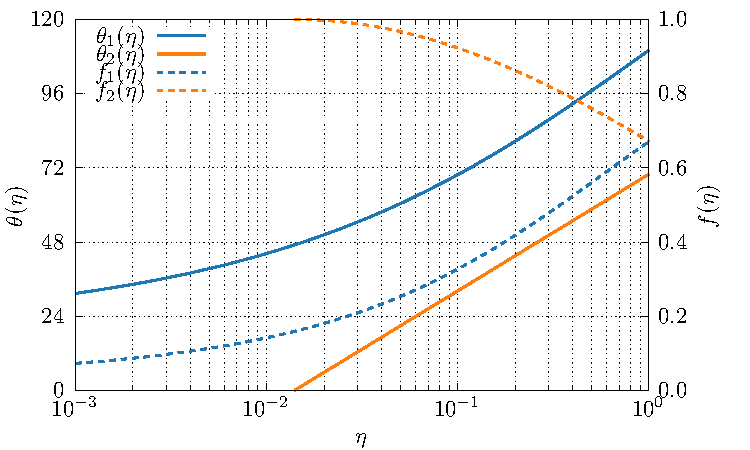
\includegraphics[]{assets/wind-shock-factor/shock-factor.pdf}
  \caption[Wind shock fraction, as a function of $\eta$]{Comparison of the opening angle of $\widetilde{S}_1$ and $\widetilde{S}_2$ as a function of $\eta$. The wind shock fraction, $f$, is also plotted. $\approx 10\%$ of the primary wind is shocked under typical WR+OB conditions, while the entire secondary wind is typically shocked.}
  \label{fig:wind-shock-factor}
\end{figure}

% Influence of orbital motion
Orbital motion is also a significant factor in the geometry of a WCR, as the stars orbit each other the WCR curves and wraps around the system, as the angle of the WCR relative to the outflow from the system is constantly changing.
The conical approximation as described in \textcite{eichler_particle_1993} was found to be valid to a distance of $r_\text{OB} \ll r \ll (P v^\infty_\text{WR})/2$, where $P$ is the orbital period.
In systems with a short orbital period, this can result in the production of a pinwheel-like structure as the WCR extends away from the stars.
In particular, the systems WR104 and WR98a produce easily observable pinwheel structures, especially in the infrared.

\subsection{Cooling in the WCR}
\label{sec:wcrcooling}
%//TODO clean up this caption
%//TODO remove grid from plot
\begin{figure}[h]
  \centering
  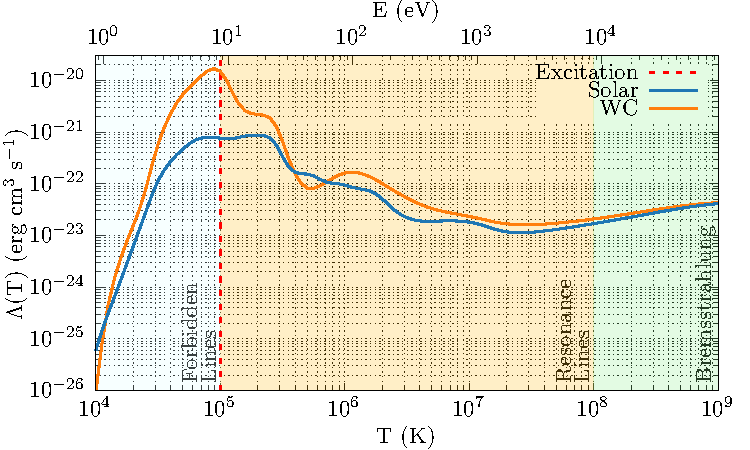
\includegraphics{assets/cooling-breakdown/cooling-curve-solar-withev.pdf}
  \caption[WC \& solar abundance plasma cooling curves]{Normalised plasma cooling rates as a function of temperature and thermal energy for solar abundance and WC abundance winds. The regions where forbidden line, resonance line and bremsstrahlung emission are dominant are highlighted, with H ionisation and recombination occuring between the forbidden and resonance line sections at $10^5$ \si{\kelvin}.}
  \label{fig:wcsolcooling}
\end{figure}

\begin{table}[h]
  \centering
  \begin{tabular}{lll}
  \\ \hline 
  \textbf{Temperature range} & \textbf{Dominant process} & \textbf{Spectral region} \\ \hline
  $\SI{5e3}{\kelvin} \lesssim T \lesssim \SI{1e5}{\kelvin} $ & Forbidden lines & IR, Optical \\
  $T \approx \SI{1e5}{\kelvin}$ & H excitation/ionisation & Optical, UV \\
  $\SI{5e3}{\kelvin} \lesssim T \lesssim \SI{1e5}{\kelvin} $ & Resonance lines & Far UV, soft X-ray \\
  $T \gtrsim \SI{1e8}{\kelvin} $ & Bremsstrahlung & Radio \\ \hline
  \end{tabular}
  \caption[Cooling processes at various temperature ranges]{Breakdown of dominant cooling processes at various temperature ranges from \cite{dysonPhysicsInterstellarMedium2021}, whilst H excitation/ionisation occurs over a very short temperature range, it is extremely influential, causing a global peak in the cooling rate at $\approx 10^5$ \si{\kelvin}. These temperature ranges are depicted in Fig. \ref{fig:wcsolcooling}.}
  \label{tab:coolprocess}
  \end{table}

% Radiative cooling, include graphs, mechanisms

Cooling due to radiation emission in a hot plasma can be broken down into a variety of processes that occur over series of temperature ranges.
Ions inside a plasma can become excited through collisions or photon absorption resulting in emission of photons as the ions de-excited. 
Mechanisms that are significant within the warm\footnote{See what I mean about the phrase ``warm''?} and hot gas phases include forbidden line emission, hydrogen excitation and ionisation, resonance lines and bremsstrahlung \parencite{dysonPhysicsInterstellarMedium2021}.
The influence of each mechanism varies over a particular temperature range, with each mechanism dominant over a certain temperature range (Table \ref{tab:coolprocess} and Fig. \ref{fig:wcsolcooling}).

% Section on forbidden line emission

The first mechanism to be discussed is forbidden line emission\footnote{Like many other phenomena discussed in this thesis, this too is a misnomer, while initially assumed to be prohibited under the contemporary understanding of atomic physics, it is in fact just astrophysicists jumping the gun again.}.
This process dominates the cooling process of cooler gas that is not fully ionised, where collisions with free electrons excite metallic elements within the gas, which de-excite through magnetic dipole and quadrupole fine structure state transitions.
This process dominates at these temperatures as the transition energies are significantly lower, on the order of \SI{1}{\electronvolt}, as the photon is also of a comparatively long wavelength, it can more easily escape from the surrounding gas.

% Section on ionisation/recombination

As the temperature increases there is a spike in the cooling rate of the gas as the hydrogen present begins to fully ionise, at this temperature a hydrogen ion and an electron may recombine, releasing a cascade of photons as the electron de-excites.

% Section on resonance line emission

As the plasma heats further resonance lines can

% Section on braking radiation

As the particle energy reaches the range of tens of \si{\kilo\electronvolt}, bremsstrahlung\footnote{Or braking radiation when you can't remember how to spell it.} becomes dominant (Fig. \ref{fig:wcsolcooling}). High velocity electrons are deflected by ions, emitting radiation in the process due to conservation of energy. 

% \parencite{1993ApJS...88..253S}
\parencite{schureNewRadiativeCooling2009}
\parencite{rybickiRadiativeProcessesAstrophysics2004}

%//TODO clean up this caption
%//FIXME use the new cooling code for this graph, early changes in ionisation fraction result in a different appearance from 1e4 to 1e6 kelvin!
\begin{figure}
  \centering
  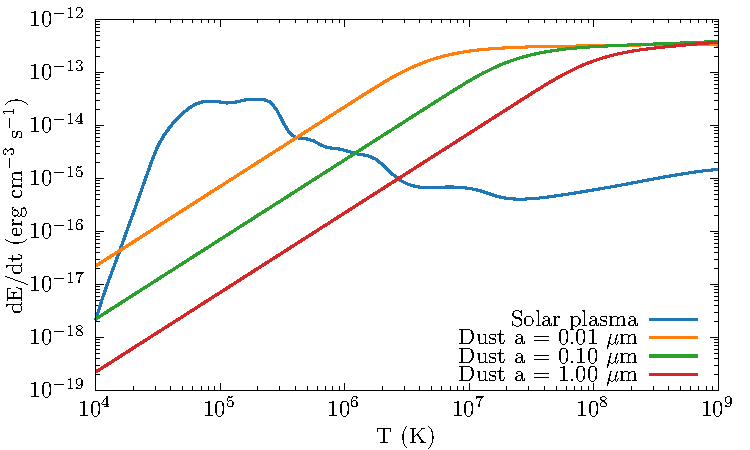
\includegraphics{assets/dust-plasma-cooling-comparison/cooling-comparison.pdf}
  \caption[Dust cooling vs. plasma cooling]{Comparison of plasma cooling to dust cooling with different grain sizes in a solar abundance gas, with a gas density of \SI{1e-20}{\gram\per\centi\metre\cubed} and a dust-to-gas mass ratio of 0.01.}
  \label{fig:dustplasmacomparison}
\end{figure}


We define an energy loss rate of a volume of gas, $\dot{E}$, which in the case of plasma cooling is calculated by the equation:

\begin{equation}
  \frac{dE}{dt} = \left(\frac{\rho}{m\rms{H}}\right)^2 \Lambda(T) = n\rms{g}^2 \Lambda(T)
\end{equation}
\noindent
where $n\rms{g}$ is the number density of the gas and $\Lambda(T)$ is the emissivity of the gas.
The gas is assumed to be optically thin.

% Needs to be spun off into a subsection

Radiative cooling through plasma and dust cooling can play an extremely important role in the dynamics of the WCR.
A more radiative WCR will typically be dominated structurally by thermal and thin-shell instabilities, leading to regions with markedly higher local gas densities.
In addition to these instabilities, the region will overall be significantly more dense, as a radiative shock is capable of compressing gas beyond the adiabatic limit of $\rho\rms{post-shock} = 4 \rho\rms{pre-shock}$. 
The post-shock region will also be much cooler, as gas can cool back to the initial wind temperature.
This allows dust to form, and is perhaps the most important factor for explaining dust formation in a CWB system.
The influence on radiative cooling varies from system to system, but the influence is determined exclusively by the wind properties and orbital separation of the system, leading to it being consistent in systems with circular orbits, and can vary significantly in the case of systems with highly elliptical orbits.
This provides further clues for the mechanisms behind the formation of dust in the WCR, as we shall see later.
The extent to which the WCR is affected by cooling is dependent on similar parameters that govern the shape and structure of the WCR itself.
Cooling becomes influential on the structure of the WCR if the immediate post-shock gas is able to cool to the post shock temperature shortly after escaping from the shock, this is described in this thesis as:

\begin{equation}
  \chi = \frac{\tau\rms{cool}}{\tau\rms{esc}} ,
\end{equation}

\noindent
where $\tau\rms{cool}$ is the cooling timescale and $\tau\rms{esc}$ is the escape timescale.
The cooling timescale is the time required for the gas to radiate all of its energy at a rate $\dot{E}$, hence, $\tau\rms{cool} = E/\dot{E}$ or:

\begin{equation}
  \label{eq:taucool}
  \tau\rms{cool} = \frac{k\rms{B}T\rms{s}}{4n\rms{w}\Lambda(T\rms{s})},
\end{equation}

\noindent
where $k\rms{B}$ is the Boltzmann constant, $T\rms{s}$ is the shock temperature and $n\rms{w}$ is the post-shock wind number density.
The escape timescale represents the approximate time taken for the gas to escape the shock, corresponding to:

\begin{equation}
  \label{eq:tauesc}
  \tau\rms{esc} = \frac{d\rms{sep}}{c\rms{s}} , 
\end{equation}

\noindent
where $c\rms{s}$ is the post-shock sound speed.
As the expected shock temperatures of a CWB align closely with a local minima in $\Lambda(T)$, $\chi$ can be approximated with the equation:

\begin{equation}
  \label{eq:coolingparameter} 
  \chi \approx \frac{v^4_{\infty,8} d_\text{sep,12}}{\mdot_{-7}},
\end{equation}

\noindent
where $v_{\infty,8}$ is the wind terminal velocity in units of \SI{1e8}{\centi\metre\per\second}, $d_\text{sep,12}$ is the separation distance in units of \SI{1e12}{\centi\metre} and $\mdot_{-7}$ is the mass loss rate in units of \SI{1e-7}{\solarmass\per\year}
\parencite{stevens_colliding_1992}.
In the case of a CWB system with a cooling parameter $\chi \gg 1$, the system is adiabatic, leading to smooth winds and gas remaining at high temperatures, at it can only cool through expansion.
In the case of $\chi \leq 1$, the system is strongly radiative, the gas rapidly cools after being shocked, leading to a very dense post-shock region with a structure strongly influenced by thermal instabilities.

As we can see from Eq. \ref{eq:coolingparameter}, we find that strongly radiative WCRs are favoured in stars with stars with slow, dense winds and close orbits.
Wind velocity in particular is highly influential on the radiative dynamics of the WCR, and could be one of the driving reasons for a lack of dust formation in certain WC sub-types.
Systems with high eccentricities can also vary their orbit significantly, leading to fluctuations in $\chi$ by 2 orders of magnitude.
The corresponding velocity shear between a WR and an OB wind also results in the formation of Kelvin-Helmholtz instabilities.

\subsubsection{Dust cooling}

% Dust cooling? Might need to move CWB dust formation up
The presence of dust within the immediate post-shock environment significantly increases the cooling rate.
Fig. \ref{fig:dustplasmacomparison} compares rate of cooling due to dust emission of various types of grains to plasma cooling at solar abundances, 
As $\Lambda_g$ and $\Lambda_D$ are both proportional to $\rho_g^2$, dust cooling will dominate at high temperatures so long as there is sufficient amounts of dust.
%//TODO Lengthen paragraph, introduction to dust cooling

As dust grains collide with ionised gas and electrons, this imparts kinetic energy into the grains, heating them and causing them to emit infrared radiation. Assuming that there is a net accretion of ions and electrons onto the dust grains and the gas is optically thin in the infrared regime, energy is efficiently removed from the gas.
At particularly high temperatures this effect can dominate over high-temperature plasma cooling processes such as bremsstrahlung, as seen in Fig. \ref{fig:dustplasmacomparison}.
Fig. \ref{fig:collisionalheatingcomparison} compares dust grain heating rates due to electron and ion collisional excitation in a solar abundance and WC abundance flow.
At lower temperatures the dust grain cooling rate is dominated by electron excitation, especially in the WC case as the ratio of free electrons to ions is significantly higher, as the WC flow is enriched by heavier elements.
However, as the grain temperature increases, collisional heating due to ions becomes more prevalent as the electrons are sufficiently energetic to pass through the grain without significant energy transfer; this is referred to as the electron transparency, $h_e$ \parencite{dwek_infrared_1981}.

\begin{figure}[h]
  \centering
  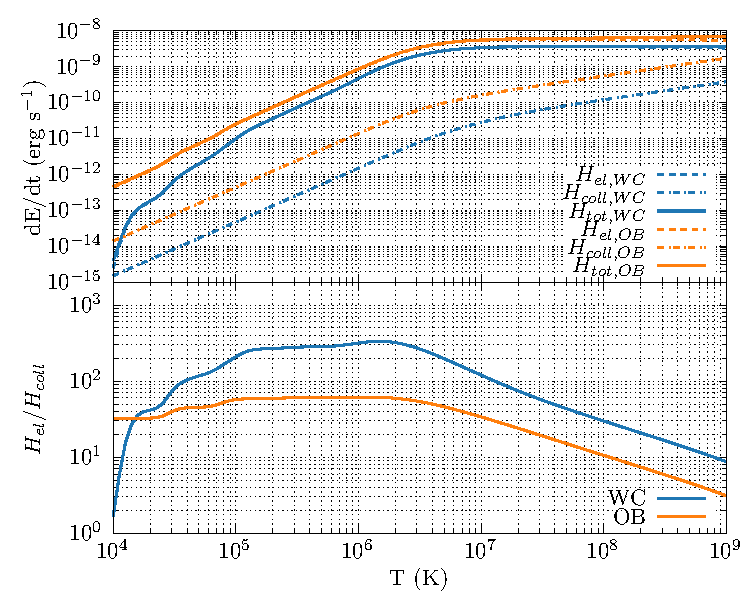
\includegraphics{assets/dust-electron-contribution/coll-el-comp.pdf}
  \caption[$H_{el}$ and $H_{coll}$ comparison]{Comparison of grain heating rate due to ion collisional excitation, $H_{coll}$, and electron excitation, $H_{el}$. The dust grain has a grain radius of \SI{5e-3}{\micro\metre} and is travelling through a gas with a density of $10^{-20}$ \si{\gram\per\centi\metre\cubed} with solar and WC abundances.}
  \label{fig:collisionalheatingcomparison}
\end{figure}

Work by \cite{dwek_infrared_1981} is used predominantly in this project to simulate cooling due to dust, a fast method for calculating the cooling rate due to dust was integrated into the numerical code for this project, which is elaborated on in section \ref{sec:dustcoolingmodel}.
% Finish and link to below paragraph

%Find citation for spitzer 1978

The heating rate of a dust grain due to collisions 

\begin{equation}
  \begin{split} 
      H_\text{coll} = & n \pi a^2 \langle Q(E,q,U) \rangle \\
      & \times \langle v (E-qU) f(a,E-qU) f(a,E-qU) \rangle \, \si{\erg\per\second}
  \end{split}
\end{equation}

%Explain constants
This can be simplified and expressed in the equation:

\begin{equation}
  \begin{split}
    H_\text{coll} & = \left(\frac{32}{\pi m}\right)^{1/2} n\pi a^2 (k_B T)^{3/2} h(a,T) \\
    & = \num{1.26e-19} \frac{n}{A^{1/2}} a^2 (\si{\micro\metre}) T^{3/2} h(a,T) \, \si{\erg\per\second}
  \end{split}
\end{equation}

% This part is very dry and is going to explain the equations more in depth
% Main source will be dwek 1981 appendix 2



% Instabilities due to cooling, might spin off into it's own appendix chapter?
% Theres a particular paper that covers this 
% Mainly need to discuss KH instabilities, and how they relate to cooling



\subsection{Dust formation in CWB systems}
\label{sec:cwbdust}

%Intro to dust formation in said systems
Despite the extremely violent conditions thus far described in CWB systems, these systems appear to be extremely prolific producers of interstellar dust.
Whilst single star WC systems can produce small amounts of dust in the form of amorphous carbon grains (though this could be observed to be extremely rare, pending the results of \textcite{medinaAreAllWCd2021}), binary systems have been observed to convert up to $10^{-3}$ of their wind masses from ionised carbon into amorphous carbon dust grains, this results in a typical dust production rate of $10^{-8} \, \si{\solarmass\per\year}$, on part with a typical AGB star.
This dust forming behaviour has only been observed in particularly energetic WC stars (predominantly WC9, with some WC7-8 examples), WN and WO systems have not been observed producing dust, this is most likely due to amorphous grains being significantly more chemically stable and resilient to effects such as sublimation and photoevaporation than water ice or silicate grains \parencite{salpeter_formation_1977,draineDestructionMechanismsInterstellar1979}.
Dust formation is also observed to form within the WCR, which can form quite beautiful pinwheel-shaped patterns, as dust streams away from the stars in the post-shock outflow.

\begin{table}[]
  \centering
  \begin{tabular}{ccccccc}
    & \multicolumn{2}{c}{Persistent} & \multicolumn{2}{c}{Variable} & \multicolumn{2}{c}{Episodic} \\ \cline{2-7} 
    & Total & Example & Total & Example & Total & Example \\ \hline
   WC4 & 1 & WR19 & 0 & --- & 0 & --- \\
   WC5 & 0 & --- & 0 & --- & 1 & WR47C \\
   WC6 & 1 & WR124-10 & 0 & --- & 0 & --- \\
   WC7 & 3 & WR102-22 & 0 & --- & 4 & WR140 \\
   WC8 & 6 & WR13 & 1 & WR48a & 3 & WR122-14 \\
   WC9 & 45 & WR104 & 6 & WR98a & 1 & WR75-11 \\ \hline
   Total & 56 &  & 7 &  & 9 &  \\ \hline
  \end{tabular}
  \caption[Numer of confirmed WCd systems]{Number of confirmed WCd systems with known spectral type and dust formation type from the Galactic Wolf-Rayet Catalogue \parencite{rossloweSpatialDistributionGalactic2015}, systems with uncertain spectral types not included, while systems labelled ``d'' are included within the ``persistent'' category for their associated spectral type.}
  \label{tab:wc-summated-list}
\end{table}

% Rarity
Whilst beautiful, Wolf-Rayet systems are elusively rare.
The Galactic Wolf-Rayet Catalogue\footnote{The most recent version of this catalogue is available at \texttt{\href{http://pacrowther.staff.shef.ac.uk/WRcat}{http://pacrowther.staff.shef.ac.uk/WRcat}}} \parencite{rossloweSpatialDistributionGalactic2015} has a collection of 667\footnote{At time of time of writing, with the last update being August 2020.} known galactic WR stars, 106 of such stars are contained within a binary system, with 41 such binaries containing WC stars.
\textcite{rossloweSpatialDistributionGalactic2015} notes that there are a total of 42 confirmed WCd systems, approximately 35\% of all WC systems, though this value is somewhat out out date and includes single star systems.
A more up-to-date estimate performed for this thesis using the updated dataset estimates a total of 80 WCd systems, of which 72 have well-determined spectral subtypes (table \ref{tab:wc-summated-list}).
% Impact of systems 
\textcite{rossloweSpatialDistributionGalactic2015} goes on to estimate that out of an estimated total of 1900 galactic WR stars, approximately 300 of these stars are predicted to be dusty WC stars.
Whilst this is a far cry from the number of galactic AGB stars - of which carbon-rich AGBs outnumber WCd stars by approximately 3 orders of magnitude \parencite{ishiharaGalacticDistributionsCarbon2011} - these systems can still significantly impact the surrounding interstellar medium, with strong stellar feedback propagating large quantities of dust into the surrounding medium.

% Number of WCd systems, reasoning for only certain subtypes being dust forming
Table \ref{tab:wc-summated-list} contains an excerpt of the observed WCd systems with clearly defined spectral subtypes, most dust producing stars are either WC8 or WC9 subtypes, which are markedly cooler and less luminous than their WC4 counterparts.
This reduced luminosity is potentially the driving factor for dust formation in the system.
As WC8-9 systems have slower, cooler winds \parencite{niedzielskiKinematicalStructureWolfRayet2002}, they are more strongly influenced by post-shock cooling, allowing for greater dust formation within the WCR.
A small number of these systems have somewhat variable or episodic dust production cycles, such as WR98a and WR140, which are the two systems being observed within this thesis.
Furthermore, the bulk of WCd systems do appear to be in binary systems with a close periastron passage, in fact, this orbit itself appears to be a driving force behind how dust is produced in these systems, as we will later discuss.

%Theories as to why
A good starting point to understanding dust formation is to understand how the WCR can mitigate the mechanisms resulting in dust destruction, whilst aiding the processes involved in dust formation.
As previously discussed, dust can be destroyed through high-velocity collisions with grains, as well as evaporation through heating or ionising radiation.
These processes are mitigated through the cooling, as well as the high level of UV extinction due to the high density of the WCR.
Meanwhile, the dust production rate increases within high density regions, as collisions between dust grains and gas occur at a much higher rate.
The same can be said with dust grains, allowing for fast growth from gas and impinging ion accretion, and grain-grain collision as the number density of dust grains begins to increase.
The accumulation of these effects would be a very fast initial growth rate, which tapers off as the post-shock region diffuses and expands, resulting in a reduction in density.

% Role of instabilities
The presence of instabilities driven by cooling and other factors can lead to pockets of high density post-shock material, as high density drives dust formation, this can lead to ``clumps'' of highly dust-enriched post-shock stellar wind.
These clumps would have additional protection from UV photons, and would also be cooled enough for dust to form, thus, the driving hypothesis for this theory is that these are regions where the bulk of dust formation would occur.
% How to make lots of dust + reminder of aims of project.
As such, it is theorised in order to achieve a high rate of dust formation, a dense, highly radiative post-shock WCR must be formed, as cooling in the post-shock region is dependent on separation distance, wind velocity and mass loss rate, these parameters should first be explored, with the knowledge gleaned used to direct an analysis of observed systems such as WR140.

%Observational data Link to Crowther papers in particular, dust formations only around WC
% Discuss role of eccentricity
Eccentricity appears to play an important factor in the production of dust, highly eccentric systems can vary their dust production rates significantly.
Fig. \ref{fig:periodicmags} shows the periodic change in mid-IR emission that can be explained as dust emission from small amorphous carbon grains, in the case of systems such as WR140 or WR125 dust production can be reduced to the point where associated emissions can drop by several magnitudes.
This relation is clearly periodic, with a peak in dust production production coinciding with the periastron passage of these systems.
This implies that dust production is dependent on orbital separation, which will influence the degree of cooling occurring within the WCR, it could potentially also alter the wind velocity on collision, which will also influence dust production in the same manner.
% Metastudy
Further analysis of available dust producing CWB systems suggests that \textit{all} WCd systems with circular orbits produce dust either persistently or with a degree of variability, while eccentric WCd systems are solely produce dust episodically.

\begin{figure}
  \centering
  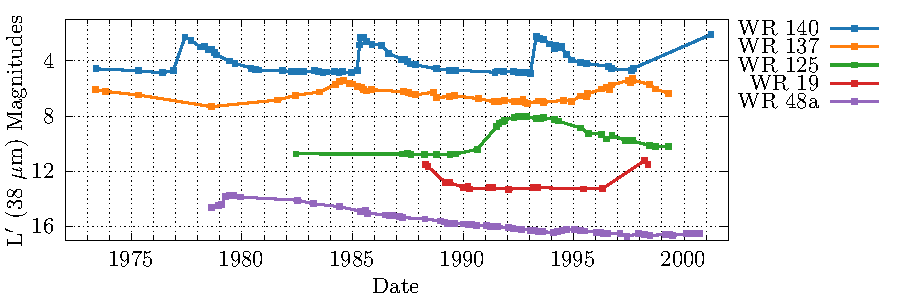
\includegraphics[]{assets/magnitudes/magnitudes.pdf}
  \caption[L$^\prime$ photometry of episodic dust making stars]{L$^\prime$ photometry for episodic dust making stars, data derived from \textcite{crowther_dust_2003}, and provided by PM Williams in private correspondence. WR 140 and WR 137 in particular have extremely predictable dust forming events which correspond to periastron passage in both systems.}
  \label{fig:periodicmags}
\end{figure}


\subsection{Important WCd systems}

The principle systems that are being observed in this thesis are the variable dust forming system, WR98a, and the episodic dust forming system WR140.
The archetypal continuous dust forming system WR104 was also proposed for simulation, but had to be cut due to time constraints, this system will also be discussed to provide a point of comparison between the two systems.

\begin{table}[h]
  \centering
  \begin{tabular}{cccccccc}
  \hline
  System & $\dot{\text M}_{\text{WR}}$ & $\dot{\text M}_{\text{OB}}$ & $v_{\text{WR}}^\infty$ & $v_{\text{OB}}^\infty$ & $\eta$ & $\chi_\text{min}$ & $\dot{\text M}_\text{D}$ \\
   & (\si{\solarmass\per\year}) & (\si{\solarmass\per\year}) & (\si{\km\per\second}) & (\si{\km\per\second}) & (AU) & & (\si{\solarmass\per\year}) \\ \hline
  WR98a & \num{5.0e-6} & \num{5.0e-8} & 900  & 2000 & 0.0222 & 0.7970 & $\left(6.10^{+1.77}_{-1.38}\right) \times 10^{-7}$ \\ 
  WR104 & \num{3.0e-5} & \num{6.0e-8} & 1220 & 2000 & 0.0033 & 0.2430 & $\left(4.39^{+1.27}_{-0.97}\right) \times 10^{-6}$ \\
  WR140 & \num{5.6e-5} & \num{1.6e-6} & 2895 & 3200 & 0.0314 & 2.6866 & $\left(8.11^{+4.83}_{-4.15}\right) \times 10^{-10}$ \\ \hline
  \end{tabular}
  \caption[Wind properties of systems considered for simulation]{Wind properties of systems considered for simulation in this thesis.}
  \label{tab:systems-wind-properties}
\end{table}

\begin{table}[h]
  \centering
  \begin{tabular}{ccccccccc}
  \hline
  System & Classification & Period & Eccentricity & Inclination & $M_{\text{WR}}$ & $M_{\text{OB}}$ & Periastron & Apastron \\
   & & (d) & ($e$) & ($i$) & (\si{\solarmass}) & (\si{\solarmass}) & (AU) & (AU) \\ \hline
  WR98a & WC8-9+OB & 556 & $\sim 0$ & $35\pm6^\circ$ &10.0 & 18.0 & 4.06 & 4.06 \\
  WR104 & WC9d+B0.5V & 245 & 0.0600 & $\lesssim 16^\circ$ & 10.0 & 20.0 & 2.20 & 2.48 \\
  WR140 & WC7+O5 & 2869 & 0.8993 & $119.1\pm0.9^\circ$ & 10.31 & 29.27 & 1.53 & 26.9 \\ \hline
  \end{tabular}
  \caption[Orbital properties of systems considered for simulation]{Orbital properties of systems considered for simulation in this thesis.}
  \label{tab:systems-orbital-properties}
\end{table}

\subsubsection{WR98a}

\begin{figure}
  \centering
  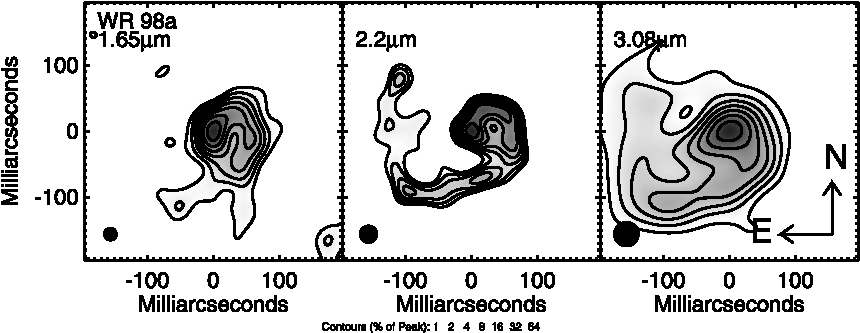
\includegraphics{assets/systems/wr98a-monnier2007.pdf}
  \caption[\textit{Multiwavelength image of WR98a \parencite{monnierKeckAperturemaskingExperiment2007}}]{Multiwavelength aperture synthesis images of WR98a taken on June \nth{24} 2000, at 1.65, 2.2, and \SI{3.08}{\micro\metre}. Plot sourced from \textcite{monnierKeckAperturemaskingExperiment2007}, the significant IR excess is a clear sign of ongoing dust production. The system also has a pronounced pinwheel structure most prominent at \SI{2.2}{\micro\metre}.}
\end{figure}

% Physical properties

WR98a is a WC8-9+OB variable dust formation system.
It is has an approximately circular orbit with a semi-major axis of \SI{4.06}{\au}, and is inclined at $\approx 35^\circ$ from Earth.


% Historical observation 

\parencite{monnierPinwheelNebulaWR1999}


% Hendrix paper dust formation monnier 2002 radio domain

% Ease of simulation, good starting point
WR98a was chosen for simulation primarily due to its moderate rate of dust formation, and comparatively docile winds.
With a a slow WC wind velocity of \SI{900}{\kilo\metre\per\second} and a WC mass loss rate of \SI{5e-6}{\solarmass\per\year}



The dust formation rate is lower than many WC systems \parencite{lauRevisitingImpactDust2020}

Due to these factors the system is markedly easier to simulate, and thus provided a good starting point for our work as we refined the model and implemented features into the hydrodynamical system.

A comparatively wide orbit reduces the number of cells required to simulate the system, simplifying the simulation of the system further.

Finally, WR98a has previously been simulated using a multi-fluid dust model in \textcite{hendrix_pinwheels_2016}, this allows us to provide a point of comparison between our work and already published work.
This is especially useful as there are only a handful of papers that cover dust models in CWB systems.

% Questions as to orbit shape, approximately circular


% Parameter space exploration
Because of this relative ease of simulation and relatively slow wind velocity for both stars in the system, WR98a was chosen to be the baseline system for the research conducted in chapter \ref{chap:parameterspace}.

\subsubsection{WR140}

% Physical properties

% Historical observation
WR140 is significant in that it is the first system to be observed with episodic dust forming CWB properties, \textcite{williamsCondensationShellHD1978} notes a rapid brightening in the infrared, suggesting the formation of a new shell of dust around the system.
WR140 has undergone frequent observations, with spectroscopic data going back to 1972, and is perhaps the most well-observed episodic WCd system, for this it was immediately considered for 

% Eccentric orbit, variable dust formation

% Difficulty of simulation
As it is a highly eccentric system with a particularly long period orbit, a number of difficulties 

with the constraints of only having SMR available throughout this project, with AMR not currently being stable in this particular hydrodynamical code, 
% Snippet
As such, it was decided to only simulate the system as it undergoes closest approach, from $\phi = 0.95$ to $\phi = 1.10$, as a full orbit of the system would require AMR to undertake within the time constraints remaining in this project. 


\subsubsection{WR104}

\begin{figure}
  \centering
  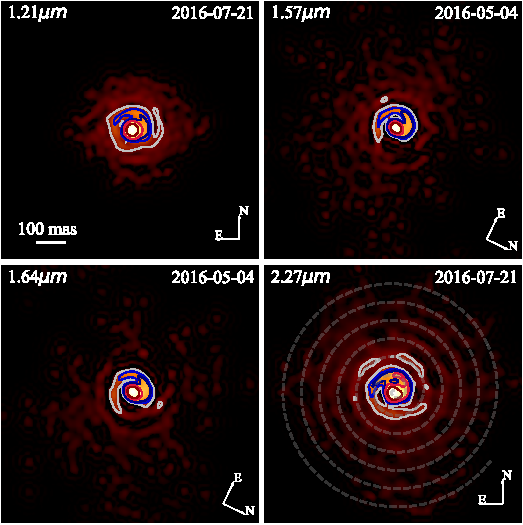
\includegraphics[]{assets/systems/soulain-2018-wr104.pdf}
  \caption[\textit{Spiral structure of WR104 \parencite{soulainSPHEREViewWolfRayet2018}}]{Deconvolution of J, H, K, and \SI{2.27}{\micro\metre} bands of WR104 sourced from \textcite{soulainSPHEREViewWolfRayet2018}. The spiral pattern and first revolution is visible in all images, in particular at \SI{2.27}{\micro\metre}.}
  \label{fig:soulain-wr104}
\end{figure}

% Physical properties
WR104 is an archetypal example of a continuous WCd system, it is a comparatively tight binary with a semi-major axis of \SI{2.34}{\au} and a period of $\sim 241$ days, the orbit is also relatively circular, with an eccentricity of $e = 0.06$ \parencite{lamberts_colliding_2012}.
The system consists of a WC9 star with a B0.5V partner \parencite{williamsSpectroscopyWC9WolfRayet2000}, this combination of a WC star and a comparatively weak B partner results in a severely imbalanced wind, with a momentum ratio of $0.003$, an order of magnitude lower than WR98a.
This imbalanced wind, combined with the tight orbit, results in an extremely strong WCR that is constantly churning out dust.
% Mass loss rate
Using radiative transfer models, \textcite{harries_three-dimensional_2004} calculated a dust production rate of \SI{8(1)e-7}{\solarmass\per\year}, corresponding to 2\% of the carbon mass loss rate of 
A more advanced model by \textcite{lauRevisitingImpactDust2020}, which is used to assess the dust formation rates of systems in this thesis, calculated the dust formation rate to be $\left(4.39^{+1.27}_{-0.97}\right) \times 10^{-6}\, \si{\solarmass\per\year}$.

% Why is it archetypal 

WR104 can be considered to be an ideal example of a continuous dust forming system, the system is relatively close, at a distance of \SI{2.5}{\kilo\parsec}, and is at an inclination that is almost face-on relative to Earth, at $i \lesssim 16^\circ$. 
As such, the pinwheel outflow from the system can be clearly resolved, with infrared excess due to dust clearly observed within the pinwheel structure (\textcite{soulainSPHEREViewWolfRayet2018}, see Fig. \ref{fig:soulain-wr104}).
Due to the systems parameters and well defined observable dusty pinwheel structure, along with prior observations and simulations of the system, it is an ideal candidate for simulation 

There are a number of reasons for this prodigious dust formation rate, as the systems orbit is comparatively close and circular with a very dense primary wind, the wind is expected to be highly radiative throughout the entire orbital period, this suggests a cool post-shock WCR that can continuously produce dust.
The estimated cooling parameter is more than an order of magnitude lower than the other systems considered for simulation, leading to a

% Why it wasn't assessed, difficulty of simulation, needed AMR
Unfortunately, despite being a very strong candidate for simulation, attempting to simulate the system proved to be exceptionally difficult.
% Many level simulation required for large-scale observation
The very close orbit of the system would mandate a very high simulation resolution, increasing the amount of compute time required to finish the simulation, only simulating a small region would prevent the pinwheel from being formed and observed, which we would have ideally wanted to include.
% Instability required running at very low Courant number
In addition the strong radiative cooling resulted in the simulation being very unstable unless the Courant number is exceedingly small, this also significantly increases compute time.
With a limited amount of compute resources as well as a limited amount of time, this stretched the feasibility of simulating this system.
% Physical effects, gayley
As the wind from the primary star is significantly stronger than its partners, WR104 has a much lower momentum ratio than the other systems being considered, as such, the WCR is situated much closer to the secondary star.
At closest approach, $r_\text{OB} \approx \SI{60}{\solarradius}$, which would require WR104 to be simulated at a much higher resolution, in turn demanding significantly more computational resources.
Physical effects, such as radiative inhibition and sudden braking may also significantly alter the wind velocity and post-shock environment, reducing the pre-shock primary wind velocity \textcite{gayley_sudden_1997}.
The pre-shock secondary wind velocity would also be influenced, due to insufficient acceleration from line driving before the winds collide.
As radiative line driving is not simulated these effects cannot be taken into account, and would have resulted in an inaccurate simulation of the system.
The effect of incomplete acceleration and sudden braking in highly wind-imbalanced systems is discussed more substantially in section \ref{sec:simassumptions}.
% Why it was discarded
With limited time remaining in the project, as well as the above factors, simulation work on WR104 was abandoned in favour of a parameter space search of a system with baseline properties similar to WR98a, as well as a limited simulation of WR140. 
Simulating this system however, is a particularly enticing avenue of future research.

\subsection{WR+WR systems}

Recently, two candidates of a theorised subset of CWB have been discovered - WR+WR systems, which have a \textit{second} Wolf-Rayet star as their partner, with a secondary wind around 3 orders of magnitude denser than a WR+OB system, this would of course result in a truly titanic wind collision.
These candidates are the recently discovered WR70-16 \parencite{callinghamAnisotropicWindsWolf2019}, and the previously discovered WR48a system \parencite{danksInfraredSpectroscopyInfrared1983}, which exhibits the spectroscopic lines of both a WC and WN system \parencite{williamsVariableDustEmission2019}.
These systems are predicted to be comparatively rare, even among CWB systems, this is largely due to unlikelihood that both stars in the system would be in their Wolf-Rayet phase at the same time.
Despite these systems having an enormous combined mass-loss rate, initial estimates of the dust production rates of both systems indicate that their dust conversion efficiencies are comparatively low compared to less energetic systems, and overall quite mundane dust production rates in general.
Whether this suppressed dust production rate is a common phenomena among WR+WR systems remains to be seen, as more systems would need to be discovered in order to determine this.

\subsubsection{WR70-16 (``Apep'') -- a recently discovered WR+WR system}

\begin{figure}
  \centering
  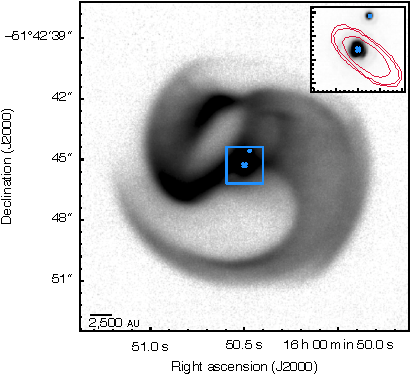
\includegraphics[]{assets/systems/apep-callingham-2019.pdf}
  \caption[\textit{VLT image of Apep \parencite{callinghamAnisotropicWindsWolf2019}}]{\textcite{callinghamAnisotropicWindsWolf2019}}
  \label{fig:apep-callingham}
\end{figure}

A potential avenue of research for this field is the simulation of WR+WR systems such as the recently discovered WR70-16 system (hereafter referred to as ``Apep''), this system was discovered due to the significant difference between the spectroscopically derived wind velocity of \SI{3400(200)}{\kilo\metre\per\second} and the observed expansion speed of \SI{570(70)}{\kilo\metre\per\second}  \parencite{callinghamAnisotropicWindsWolf2019}.
This inhibited wind velocity, far below any categorised WR wind velocity, suggests that much of the wind undergoes collision with the wind of a binary partner.
The extremely luminous non-thermal and infrared emission, suggested two extremely high mass loss rate stars within the system, as well as evidence for a third, distant partner in a loose trinary system \parencite{callinghamTwoWolfRayet2020}.
Spectroscopic analysis suggested that the central component of the Apep system consists of a nitrogen sequence WN4-6b and a carbon sequence WC8 star, with more more massive and luminous WN4-6b star kinematically dominating the system.
This discovery is very significant as it is the first galactic WR+WR system discovered, other systems have been identified, but are extragalactic in nature.

Further work by \textcite{hanExtremeCollidingwindSystem2020} has estimated the orbital parameters of Apep, finding that it is a highly eccentric system with a period of \SI{125(20)}{\year} and an eccentricity of \num{0.7(0.1)}, inclined at $\pm \ang{30} \pm \ang{5}$ towards Earth.
An initial estimate of the dust formation rate was made, finding a dust production rate of $\sim \SI{5e-7}{\solarmass\per\year}$, while observation of the surrounding dust shell suggests that it is a periodic dust forming system, which is sensible considering the systems high eccentricity.

The opening angle of the WCR was found to be very wide, at $\ang{125}\pm\ang{10}$, further suggesting the presence of two very high mass loss rate objects within the system, suggesting relatively balanced wind momenta for a CWB system.
Additional calculations by \textcite{marcoteAUscaleRadioImaging2021} estimated the systems wind momentum ratio to be $0.44\pm 0.08$, again in line with WR+WR hypothesis. 
Finally, pre-print work by \textcite{delpalacioNonthermalEmissionCollidingwind2021} finds a mass loss rate of \SI{4e-5}{\solarmass\per\year} for the WN star and \SI{2.9e-5}{\solarmass\per\year} for the WC star, which all but confirms the presence of a WR+WR binary at the heart of Apep.

With an estimated combined mass loss rate of \SI{6.9e-5}{\solarmass\per\year} we can estimate that the system has a dust conversion efficiency of 0.7\%;
whilst this system is therefore not a prodigious producer of dust this is most likely due to the extremely high wind terminal velocity and high separation distance, which would suggest a fairly smooth and adiabatic post-shock region. 
We can estimate the cooling parameter of the system to be $\sim 80$, based on angular separation from \textcite{hanExtremeCollidingwindSystem2020}, confirming that at present, the winds are adiabatic.
In order to estimate the closest approach of the system, and therefore the minimum cooling parameter an accurate measure of the stellar mass of both objects would need to be made, there is insufficient data for this at the time of writing.

\subsubsection{WR48a -- revisiting a WR+WR candidate}

% Why simulate it? And difficulties therein
WR+WR systems appear to be incredibly rare, with only a small number of extragalactic WN sequence examples in the LMC \parencite{shenarWolfRayetBinaries2019}, as well as an additional galactic WR+WR binary candidate, WR48a, \parencites(){zhekovMultiwavelengthViewDusty2014}{williamsVariableDustEmission2019}{zhekovChandraRevisitsWR2022}.
In the case of WR48a, its change in classification from a dust forming WC8 with an unknown partner to a WC8-WN8 is contemporaneous with the discovery and classification of Apep, though there is a distinct lack of recent observations of the system compared to the more recent WR+WR candidate.

\textcite{lauRevisitingImpactDust2020} calculated a dust formation rate for WR48a of $\left(8.46^{+3.48}_{-4.38}\right) \times 10^{-8} \, \si{\solarmass\per\year}$ with a dust conversion efficiency of $0.12\%$, markedly less than other systems with much less available material.
A future avenue of research would be to simulate these systems to understand why the dust formation rate is comparatively low, despite the readily available stellar material.
The main difficulty of simulating these systems is the lack of orbital parameters and accurate mass loss rates, as WR48a has insufficient data and Apep has only been recently discovered, there are currently too many unknown factors in order to build an adequate simulacrum of the systems\footnote{A lack of accurate orbital parameters is also an issue in devising simulations for more conventional WR+OB systems}.
Another difficulty is the large degree of orbital separation, high eccentricity and long orbital timescales required to simulate these systems.
The current limitations of the hydrodynamical code being used in this project render it difficult to simulate entire orbital passes of highly elliptical systems with long periods, if these issues are resolved in later versions of the hydro code however, this would present an interesting avenue of future research.
